\documentclass[10pt]{article}

% Packages
\usepackage[a4paper,margin=1in]{geometry}
\usepackage{hyperref}
\usepackage{fancyhdr}
\usepackage{setspace}
\usepackage{graphicx}
\usepackage{float}
\usepackage{amsmath}
\usepackage{amssymb}
\usepackage{color}
\usepackage{tikz}
\usetikzlibrary{shapes.geometric, arrows}
\tikzstyle{startstop} = [rectangle, rounded corners, minimum width=2cm, minimum height=0.8cm, text centered, text width=1.8cm, draw=black, fill=magenta!30, font=\tiny]
\tikzstyle{io} = [trapezium, trapezium left angle=70, trapezium right angle=110, minimum width=2cm, minimum height=0.8cm, text centered, text width=1.8cm, draw=black, fill=teal!30, font=\tiny]
\tikzstyle{process} = [rectangle, minimum width=2cm, minimum height=0.8cm, text centered, text width=1.8cm, draw=black, fill=orange!30, font=\tiny]
\tikzstyle{decision} = [diamond, minimum width=2cm, minimum height=0.8cm, text centered, text width=1.8cm, draw=black, fill=cyan!30, font=\tiny]
\tikzstyle{arrow} = [thick,->,>=stealth]


\usepackage[
  style=apa,
  backend=biber
]{biblatex}
\addbibresource{../master thesis.bib}

% Header setup
\pagestyle{fancy}
\fancyhf{} % clear default
\lhead{{\today}}
\rhead{Salome Bachmann}
\cfoot{\thepage}

% Optional: line under header
% \renewcommand{\headrulewidth}{0.4pt}

% Remove any automatic title page
\setlength{\parindent}{0pt}
\setlength{\parskip}{\baselineskip}

\begin{document}

% If you want a title *inline*, not a title page:
{\centering \Large \textbf{Literature Review for Master Thesis}\par}

\section{Nomenclature}
Symbols, definition and unit 
\begin{description}
  \item[$\boldsymbol{t_o}$]: Subfault onset time [s], e.g. $t_o=(x-x_{\rm start})/v_{\rm rupture}$.
  \item[$\boldsymbol{x},\,\boldsymbol{x}_{\rm start}$]: Horizontal coordinate and rupture starting position [m].
  \item[$\boldsymbol{v}_{\rm rupture}$]: Prescribed rupture propagation speed [m s$^{-1}$].
  \item[$\boldsymbol{t}_{rise}$]: Rise time of a subfault/source [s].
  \item[$\boldsymbol{\Delta x}$]: Subfault width or discretisation length in x [m].
  \item[$\boldsymbol{x}_{\rm slip}$]: Prescribed slip on a subfault [m].
  \item[$\boldsymbol{M}_0$]: Scalar seismic moment per subfault [N m].
  \item[$\boldsymbol{m}_{ij}$]: Moment tensor components [N m]. 
  \item[$\boldsymbol{r}_{\rm mode}$]: Mode mix parameter [dimensionless].
  \item[$\boldsymbol{l}_{cz}$]: Cohesive process (fracture) zone length [m].
  \item[$\boldsymbol\tau_s$]: Shear strength of interface [Pa].
  \item[$\boldsymbol{l}_{ch}$]: Irwin characteristic length [m].
  \item[$\boldsymbol{\lambda}_{\min}$]: Shortest wavelength to resolve [m].
  \item[$\boldsymbol{v}_{\min},\,\boldsymbol{v}_{\max}$]: Minimum and maximum relevant wave speeds in the model [m s$^{-1}$].
  \item[$\boldsymbol{\Delta t}$]: Time step [s] for explicit time integration.
  \item[$\boldsymbol{\xi}$]: Normalized opening [dimensionless].
  \item[$\boldsymbol{\delta}$]: Local opening (separation) displacement across the interface [m].
  \item[$\boldsymbol{\delta}_c$]: Mixed-mode critical opening [m] used to nondimensionalize openings.
  \item[$\boldsymbol{\delta}_{n,c},\,\boldsymbol{\delta}_{s,c}$]: Single-mode critical openings for Mode I (normal) and Mode II (shear) [m].
  \item[$\boldsymbol{T}(\boldsymbol{\xi})$]: Cohesive traction as a function of normalised opening [Pa or N m$^{-2}$].
  \item[$\boldsymbol{T}_{\mathrm{peak}}$]: Peak cohesive traction [Pa].
  \item[$\boldsymbol{\phi}(\boldsymbol{\Delta})$]: Mixed-mode cohesive potential [J m$^{-2}$] with $\Delta=(\Delta_n,\Delta_t)$.
  \item[$\boldsymbol{\Delta}_n,\,\boldsymbol{\Delta}_t$]: Normal and tangential separations [m].
  \item[$\boldsymbol{\delta}_n,\,\boldsymbol{\delta}_t$]: Normal and tangential length scales in the cohesive potential [m].
  \item[$\boldsymbol{q}$]: Coupling parameter in the mixed-mode cohesive potential [dimensionless].
  \item[$\boldsymbol{\phi}_n,\,\boldsymbol{\phi}_t$]: Work (energies) of separation for pure normal and tangential modes [J m$^{-2}$].
  \item[$\boldsymbol{\sigma}_{\max},\,\boldsymbol{\tau}_{\max}$]: Peak normal strength and peak shear strength [Pa]. 
  \item[$\boldsymbol{\sigma}_n,\,\boldsymbol{\tau}_s$]: Normal and shear strength [Pa].
  \item[$\boldsymbol{G}_I,\,\boldsymbol{G}_{II}$]: Fracture energies for Mode I and Mode II [J m$^{-2}$].
  \item[$\boldsymbol{v}_s,\,\boldsymbol{v}_p$]: Pressure and Shear seismic wave speeds [m s$^{-1}$].
  \item[$\boldsymbol{\rho}$]: Mass density [kg m$^{-3}$].
  \item[$\boldsymbol{\mu},\,\boldsymbol{\lambda}$]: Lamé parameters [Pa].
  \item[$\boldsymbol{E}$]: Young's modulus [Pa].
  \item[$\boldsymbol{l}_{crack},\,\boldsymbol{x}_0$]: Local crack process length and initial crack front position [m] used in local coordinate definitions.
\end{description}


\section{Introduction for Thesis}

%\begin{itemize}
  %\item \textbf{General Introduction:} what are avalanches, how do they form? \par

Snow avalanches are a major natural hazard in mountainous regions; they endanger human life as well as infrastructure \parencite{schweizerSnowAvalancheFormation2003}. The Swiss Institute for Snow and Avalanche Research has reported an average of 22 fatalities caused by avalanches every year, with the number of non-fatal accidents being tenfold higher \parencite{LongtermStatistics}. These data show that avalanches are a significhant threat, which is why it is crucial to understand how avalanches form and propagate in order to protect people and infrastructure better.

  Avalanches are rapid masses of snow that move down mountain slopes due to gravity \parencite{anceySnowAvalanches2001}. Snow avalanches can either be loose snow, which starts from a point in a cohesionless surface, wet snow, or snow slab avalanches \parencite{schweizerSnowAvalancheFormation2003}. In this Master Thesis, the focus will be on dry snow slab avalanches, so mostly coherent masses of snow which contain no liquid water. Snow slab avalanches consist of a cohesive slab of snow \parencite{schweizerSnowAvalancheFormation2003} that is released because of loading at the surface, which triggers crack propagation in a weak layer \parencite{gaumeSnowFractureRelation2017a}. Weak layers are characterized by the grain shape of snow, which leads to lower cohesion of those layers \parencite{fohnMechanicalStructuralProperties1998}. 

  %\item \textbf{Relevance:} Why model avalanches? \par

As mentioned, avalanches are a major threat to human life in mountainous regions, which is why detecting the breakoff of the snow slab is important for hazard mitigation. Detecting the breakoff of the slab means that warnings can be issued in lower parts of the mountain that an avalanche is possible. Furthermore, detecting slab breakoff with DAS is also important to further understand crack dynamics in snow as well as the factors influencing crack propagation. \par

  %\item \textbf{Motivation:} why avalanches \& DAS, how is this different from papers discussed in introduction \par
  
  In this master's thesis, the aim is to detect avalanche slab breakoff and crack propagation using modeled data from distributed acoustic sensing (DAS) cables. \par

  In this thesis, a fibre-optic cable installed on the slope is treated as a continuous seismic sensor, so that deformation can be observed along its full length rather than at only a few isolated stations \parencite{parkerDistributedAcousticSensing2014}. This is possible because DAS sends optical pulses through the fibre and records the backscattered light from every position along the cable \parencite{shatalinInterferometricOpticalTimedomain1998}. Ground motion near the cable, for example weak-layer failure or slab breakoff, changes the fibre strain, which appears as phase variations in the backscattered signal \parencite{hartogIntroductionDistributedOptical2017}. The phase variations are then converted into dynamic strain and from strain, into deformation along the cable \parencite{trabattoniStrainDisplacementUsing2023}. \textcolor{magenta}{mention also the cable location here, length etc} \par 

  
  A pilot early-warning system using distributed acoustic sensing has been implemented in Norway, where avalanches are detected by their seismic signature \parencite{turquetAutomatedSnowAvalanche2024}, meaning when the avalanche is already moving downhill. Such sensors are also located in Vallée de la Sionne in the Swiss Alps \parencite{paitzPhenomenologyAvalancheRecordings2023}. The detectability of avalanches by DAS has also been studied in the Swiss Alps by \cite{paitzPhenomenologyAvalancheRecordings2023} and \cite{edmeFiberopticDetectionSnow2023}, but the detectability of the slab breakoff itself has not been studied. 

  %\item \textbf{Modeling methods:} Introduce snowpack/crocus, why are they relevant, why will they not be used, introduce MPM, DEM, advantages \& disadvantages, introduce salvus and why is this needed \par
  
   %\item \textbf{Previous models:} Introduce previous models, methods used, limitations \& further developmemts \par
  
A multitude of models are used to study different processes in snow. The SNOWPACK and CROCUS models used in the Swiss and French alps model the structure and evolution of snow \parencite{brunNumericalModelSimulate1992,barteltPhysicalSNOWPACKModel2002}. These models were developed to understand how snow evolves under different conditions, for example a changing temperature gradient and water content and what consequences this has for the formation of weak layers where failure likely occurs and avalanches are triggered \parencite{brunNumericalModelSimulate1992,barteltPhysicalSNOWPACKModel2002}. SNOWPACK and CROCUS are comprehensive models that take into account multiple governing equations and processes and what consequences they have for the structure of snow. While it is important to understand the influences on for example temperature gradient on the snow structure and weak layer formation and stability as a consequence, this is not the focus of the thesis. This is because these models are too complex and comprehensive for the purpose of trying to detect slab breakoff in DAS data as they model the entire snow structure. Using SNOWPACK or CROCUS to investigate how different snowpack compositions and factors influence the DAS signal is beyond the scope of this thesis. \par

To model crack propagation in snow, multiple numerical modeling methods have been used. \cite{cundallDiscreteNumericalModel1979} developed the distinct element method  (DEM) for granular media. This model discretizes the domain as spheres and disks, which interact with each other based on Newton's second law \parencite{cundallDiscreteNumericalModel1979}. The interactions of particles are modeled by the governing equations and the resulting forces and displacements \parencite{cundallDiscreteNumericalModel1979}. This method has been used by \cite{bobillierMicromechanicalModelingSnow2020,bobillierNumericalInvestigationCrack2024,mulakNumericalInvestigationMixedmode2019} and many others to model crack propagation and its influencing factors. The main limitation of DEM is that the particle contacts and the corresponding equations need to be recalculated every time a grain contact is made or broken \parencite{cundallDiscreteNumericalModel1979}. This means that for large, slope-scale simulations, this method becomes increasingly computationally expensive. In addition to the high computation cost, DEM also cannot account for anticrack propagation, the closure of cracks in this propagation mode is accounted for by manually removing elements from the mesh, which is not very efficient \parencite{gaumeInvestigatingReleaseFlow2019}. \par

This problem is solved by using the material point method (MPM). In this method, the material is discretized in a set of Lagrangian points, which are used to track mass, deformation and momentum \parencite{bardenhagenMaterialpointMethodGranular2000}. Because the points are not fixed, an Eulerian background mesh is needed to calculate spatial derivatives \parencite{bardenhagenMaterialpointMethodGranular2000}. This method is not only more computationally efficient on the slope-scale, it can also account for anticrack behavior and strain softening of snow \parencite{gaumeInvestigatingReleaseFlow2019}. This is why the material point method will also be used in the thesis to investigate slab breakoff in DAS data on a large scale. The material point method has been used by \cite{bergfeldSignaturesSubRayleighSupershear2025}, who modeled slope-scale experiments to understand the transition of crack propagation modes, \cite{trottetTransitionSubRayleighAnticrack2022} who modeled propagation saw tests to observe transitions in crack propagation speeds, as well as \cite{gaumeInvestigatingReleaseFlow2019} and \cite{gaumeDynamicAnticrackPropagation2018}. \par


  %\item \textbf{Crack Propagation:} intro to modes of crack propagation, where and how cracks propagate, influencing factors like snow properties, slope angle etc, cracking modes transitions \& influences on transitions \par
  
  While it is important to understand the different modeling methods and their limitations, it is also important to understand the different types of crack propagation and what factors influence them. Understanding how fast a crack can propagate and which factors influence this is important for warning, as it relates the time of the initial crack to the time where the slab breaks off depending on snow and terrain parameters.  \par

  
  Two main types of crack propagation are believed to be important for weak layer failure: anticrack propagation and shear crack propagation \parencite{bergfeldSignaturesSubRayleighSupershear2025}. There are three ways in which cracks can open up: mode I, where space is opened between the crack faces under tensile loading, and modes II and III, which represent parallel shearing and diagonal shearing \parencite{heierliAnticracksNewTheory2003}. In anticrack propagation, the weak layer consolidates under loading \parencite{knightSuperheatedIceTrue1972}, while cracks propagate in a combination of modes I-III \parencite{heierliAnticracksNewTheory2003}. \cite{gaumeDynamicAnticrackPropagation2018} modeled anticrack propagation induced by a propagation saw test (PST) using MPM, which showed that the scale of the simulations influences the propagation direction of the cracks. For smaller scale simulations, cracks propagate from top to bottom of a slope, whereas for slope-scale simulations, cracks propagate bottom to top, which means that remote triggering of avalanches is possible \parencite{gaumeDynamicAnticrackPropagation2018}. This is an important consideration for the thesis because it influences where the slab breakoff would be observed in terms of DAS cable location. Other models also show that the crack propagation speed of anticracks is influenced by slope angle and curvature: concave slope areas have higher propagation speeds than convex areas of the slope \parencite{gaumeInvestigatingReleaseFlow2019}. Furthermore, there is a directionality in propagation speed, simulations by \cite{gaumeInvestigatingReleaseFlow2019} show that cracks propagate twice as fast upslope than in the downslope direction, which is especially important when thinking about remote triggering. The slab breaks off when the slope angle exceeds the friction angle of the material \parencite{gaumeInvestigatingReleaseFlow2019}. Slope angle also influences which mode of crack propagation is more dominant \parencite{rosendahlModelingSnowSlab2020}. In steeper terrains, shear modes (II and III) dominate, whereas in flatter terrain, mode I dominates the crack propagation \parencite{rosendahlModelingSnowSlab2020}. The critical force, which is for example exerted by a skier, needed for weak layer failure is also dependent on slope angle; it decreases with increasing slope angle \parencite{rosendahlModelingSnowSlab2020}. Snow parameters also have an influence on this critical force, as shown by simulations by \cite{rosendahlModelingSnowSlab2020}: the thicker the slab or the higher the slab tensile strength, the better the force by the skier can be distributed on the weak layer and the more force is needed for failure. \par

 Multiple experiments and numerical models have shown that cracks can propagate faster than the elastic wave speed in snow, so-called supershear crack propagation \parencite{trottetTransitionSubRayleighAnticrack2022,bobillierNumericalInvestigationCrack2024,bergfeldSignaturesSubRayleighSupershear2025}. Understanding what causes the transition from sub-Rayleigh to supershear crack propagation is of high importance for the thesis, because it can give an estimate of whether supershear crack propagation will occur under certain conditions, which leads to faster propagation of cracks and less time between loading and slab breakoff. In MPM models of PST, \cite{trottetTransitionSubRayleighAnticrack2022} observe that the occurrence of supershear cracks is dependent on slope angle: in steeper terrains, supershear propagation was observed. This can be explained by slab bending, because in steep terrains, bending of the slab is not limited to the collapse depth of the weak layer \parencite{trottetTransitionSubRayleighAnticrack2022}. In  in steeper terrain, the slab can bend more because of the terrain angle, the additional bending increases tensile stress in the slab, which leads to faster crack propagation \parencite{trottetTransitionSubRayleighAnticrack2022}.These observations were also made by \cite{bobillierNumericalInvestigationCrack2024} as well as \cite{bergfeldSignaturesSubRayleighSupershear2025}. The release area of an avalanche is also tied to propagation speed: at supershear propagation speed, there is less crack arrest and therefore larger release areas \parencite{trottetTransitionSubRayleighAnticrack2022,bergfeldSignaturesSubRayleighSupershear2025}. This is crucial because larger release areas also mean a larger snow volume, which has more potential for damage. \par

Independent of crack propagation mode, different factors influence the speed and distance at which cracks can propagate in the weak layer before failure occurs \parencite{gaumeDynamicAnticrackPropagation2018,gaumeSnowFractureRelation2017a,gaumeModelingCrackPropagation2015}. As discussed above, slope angle and stiffness are important factors. Other factors include weak layer parameters: the weaker the weak layer, the slower crack propagation; the thicker the weak layer, the lower the crack propagation distance before failure \parencite{gaumeModelingCrackPropagation2015}. The depth of the slab also has an influence on propagation distance and speed: the thicker the slab, the larger the propagation distance and velocity \parencite{gaumeModelingCrackPropagation2015}. How fast a slab will break off is also dependent on the critical crack length needed for failure \parencite{gaumeSnowFractureRelation2017a}. If the snowpack is more stable, which is the case when the slab has a high elastic modulus or the weak layer is thicker, the critical crack length is higher \parencite{gaumeSnowFractureRelation2017a} because the snow can sustain longer cracks before it fails. A very important factor in material strength is loading rate: if loading is slow, sintering can occur \parencite{mulakNumericalInvestigationMixedmode2019}. This means that new snow contacts can form, which can strengthen the material \parencite{mulakNumericalInvestigationMixedmode2019}. This is in contrast to rapid loading, which happens for example due to a skier \parencite{mulakNumericalInvestigationMixedmode2019}. 


In order to understand how crack propagation and slab breakoff would look in DAS data, numerical modeling of the wave propagation is done. This is done in SALVUS, which is a package that uses spectral elements to model seismic wavefields \parencite{afanasievSalvusFlexibleHighperformance2017}. \par

The different snow processes described have differenit implications for the seismic wavefield, which will be modeled. Firstly, the loading which occurs before crack nucleation changes the stress state of the snowpack. The weak layer collapse and anticrack propagation produce volumetric compaction in the snowpack, this produces a seismic signal. The crack propagation, whether sub-Rayleigh or supershear, creates a moving rupture front, which can be likened to a moving source of seismic waves, the cracks itself also create a seismic signal. Lastly, the slab breakoff and sliding creates a seismic signal because a large mass of snow moves downhill, which likely creates the largest seimsic signal of all of the processes mentioned. The signals of the different processes described will be modeled in the thesis, which will help to understand how the different processes look in DAS data and whether they can be distinguished from each other. \par

  %\item \textbf{Considerations relevant for thesis}: how does scale influence models, what factors influence DAS modelling, open questions \par
  
  Based on the above information, there are multiple considerations necessary in order to model DAS data of crack propagation accurately. The scale of the models is an important factor, because as mentioned, it influences the direction of crack propagation. This influences at which location along or relative to the DAS cable slab breakoff will occur, which changes the measured data. Furthermore, multiple parameters influence the time passed between initial cracking and slab breakoff, these are important to consider when interpreting data. The different modes of crack propagation are also important to consider, it is possible that a transition between sub-Rayleigh and supershear crack propagation can be observed in the data. The loading rate can also be considered, because slower loading leads to stabilizing processes such as sintering. \par

  \textcolor{magenta}{here i elaborate the research questions, but I don't know which one I will focus on yet} 

  \begin{itemize}
      \item \textcolor{magenta}{Different DAS signatures for different propagation modes (sub-raleigh vs supershear)}
      \item \textcolor{magenta}{models based on loading rate to see if DAS data looks different}
      \item \textcolor{magenta}{Distinction of processes: Weak layer colapse, crown and staunchwall fractures}
      \item \textcolor{magenta}{Relation to snow properties in models}
      \item \textcolor{magenta}{relationship between crack propagation and release area}
  \end{itemize}

%\end{itemize}

\section{Methods}

\subsection{Wave Propagation Modeling}
The model described in \ref{sec:czm methods} is implemented using the finite-element (FE) method in SALVUS. To discretize a domain, the domain is divided into a finite number of elements \parencite{FiniteElementMethod}. The boundaries of these elements describe the mesh, the mesh has a finite number of grid-points (edge points of the elements) \parencite{FiniteElementMethod}. The governing equations are determined at every element node, so for rectangular elements with nodes 1,2,3 and 4, there is the system $\ r^1 = \begin{pmatrix}r_1^1 \\ r_2^1 \\ r_3^1\\ r_4^1 \end{pmatrix}$ for force  and $\ u^1 = \begin{pmatrix}u_1^1 \\ u_2^1 \\ u_3^1\\ u_4^1 \end{pmatrix}$ for displacement \parencite{FiniteElementMethod}. The residual or characteristic relationship of linear elastic elements is of the form $\ r^1 = f^1-K^1u^1 $, where f are the nodal forces distributing load on the nodes and K is the stiffness matrix of a specific element \parencite{FiniteElementMethod}. \par

The governing equation considered in this case is the elastic wave equation, because real-life crack propagation has p- and s-waves. The wave equation for a heterogenous elastic solid in the n-dimensional domain G is 
\begin{equation}
  \rho\delta_t^2u = \nabla \cdot \sigma + f
\end{equation} \parencite{afanasievModularFlexibleSpectralelement2019}


\subsection{Cohesive Zone Model}
\label{sec:czm methods}

The rupture model used in the simulations is implemented as a mixed-mode Cohesive Zone Model (CZM) following \cite{mahajanModelingInterfacialCrack2008}. This model was chosen because there is a narrow band ahead of the fracture zone, the cohesive zone, where the material is already weakened. This means that before a point in the material cracks, there is already weakening of the material before. This seems to be reasonable for representing crack propagation in snow, since failure occurs as a consequence of loading and is not spontaneous. The computational domain extends 400 m in the horizontal (x) direction and 3 m in the vertical (y) direction and contains a 1.5 m snow layer over a 1.5 m air layer. Material parameters for the snow layer are taken from \cite{guillemotEffectSnowfallChanges2021}. The mixed-mode behavior is implemented because in reality, crack propagation can involve both normal and shear displacement.  \par

The mesh is generated to resolve frequencies up to the 95th percentile of the source wavelet's frequency content. Cohesive tractions are prescribed on zero-thickness interface elements and depend on the normalized opening \(\xi=\frac{\delta}{\delta_c}\). The zero-thickness interface elements are implemented by not solving for volumetric strain but displacement between interfaces instead. For the linear softening law used here the traction in a given cohesive element follows
\[ T(\xi) = T_\mathrm{peak}\,(1-\xi) \quad\text{for } 0\leq\xi\leq1,\qquad T(\xi)=0\ \text{for }\xi>1, \]
where \(T_\mathrm{peak}\) is the peak cohesive traction and \(\delta_c\) the critical opening. The normalized opening can be related to the local crack coordinate as \(\xi=\frac{(x-x_0)}{l_{crack}}\) for a crack front with initial position \(x_0\) and local process length \(l_{crack}\). \par

The mixed-mode potential used in the code follows the form from \cite{mahajanModelingInterfacialCrack2008}. With $\Delta=(\Delta_n,\Delta_t)$ denoting normal and tangential separations, the potential is written as
\[
\phi(\Delta)=\phi_n\,\exp\left(-\frac{\Delta_n}{\delta_n}\right)\left\{\left[1+\frac{\Delta_n}{\delta_n}\right]+q\left[1-\exp\left(-\frac{\Delta_t^2}{\delta_t^2}\right)\right]\right\},
\]
from which the normal and tangential tractions are obtained, the implementation uses the same closed-form expressions. This is so that peak tractions occur at $\Delta_n=\delta_n$ and $|\Delta_t|=\delta_t/\sqrt{2}$. The normal and shear works of separation relate to peak strengths via
\[ \phi_n = e\,\sigma_{\max}\,\delta_n, \qquad \phi_t = \sqrt{\tfrac{e}{2}}\,\tau_{\max}\,\delta_t, \]
and the critical openings for pure modes are computed as
\[ \delta_{n,c}=\frac{2G_I}{\sigma_n},\qquad \delta_{s,c}=\frac{2G_{II}}{\tau_s}, \]
with the mixed-mode critical opening
\[ \delta_c=\sqrt{(1-r_{\rm mode})\,\delta_{n,c}^2 + r_{\rm mode}\,\delta_{s,c}^2 }\;.
\]

Lamé parameters are derived from input seismic speeds and density: \(v_s=\sqrt{\frac{\mu}{\rho}}\) so that \(\mu=\rho v_s^2\), and \(v_p=\sqrt{\frac{(\lambda+2\mu)}{\rho}}\) so that \(\lambda=\rho(v_p^2-2v_s^2)\). Young's modulus is then computed from the Lamé parameters: \(E=\dfrac{\mu(3\lambda+2\mu)}{\lambda+\mu}\) \parencite{kAkiRichards19801981}. These conversions are applied for every material in the model. \par

The critical opening distances for pure normal (Mode I) and shear (Mode II) separations are computed from the corresponding fracture energies, strenghts, and peak tractions as
\[ \delta_{n,c}=\frac{2G_I}{\sigma_n},\qquad \delta_{s,c}=\frac{2G_{II}}{\tau_s}, \]
and combined for mixed-mode behaviour using
\[ \delta_c = \sqrt{(1-r_{\rm mode})\,\delta_{n,c}^2 + r_{\rm mode}\,\delta_{s,c}^2 }, \]
where \(r_{\rm mode}\in[0,1]\) controls the mode I/II mix, where 0 is pure mode I and 1 is pure mode II. In the current implementation the slip on each subfault follows the prescribed linear slip law up to the critical slip distance. The mode mix is an user-input parameter, while all the other parameters are derived from laboratory experiments from \cite{mahajanModelingInterfacialCrack2008}.  \par

The characteristic Irwin length for shear is calculated as \(l_{ch}=\frac{E_{\rm eff}G_{II}}{\tau_s^2}\), and the cohesive zone length is taken as \(l_{cz}=\tfrac{\pi}{8}l_{ch}\), which sets the spatial extent over which cohesive weakening is active ahead of the crack tip. \par

Rupture propagation speed is chosen with respect to the local shear-wave speed and the bounds discussed in \cite{trottetTransitionSubRayleighAnticrack2022}. Where appropriate, the rupture speed is corrected for finite slab thickness and bending stiffness to account for slab flexure effects. The rupture front is discretized into a sequence of subfaults: each subfault is activated at an onset time
\[ t_o = \frac{x-x_{\rm start}}{v_{\rm rupture}}, \]
using the subfault horizontal position \(x\), the rupture starting position \(x_{\rm start}\), and the prescribed rupture speed \(v_{\rm rupture}\). \par

Each activated subfault is represented as a point/source in the SALVUS source array. The scalar seismic moment for a subfault is computed from the shear modulus, the prescribed slip, and the subfault width \(\Delta x\):
\[ M_0 = \mu\,x_{\rm slip}\,\Delta x. \]
Moment-tensor components are set according to the user-specified mode-mix ratio, e.g. here the implementation uses
\( m_{xx}=0,\; m_{xy}=M_0\,r_{\rm mode},\; m_{yy}=-(1-r_{\rm mode})M_0\),
which yields pure mode behaviour at the extremes of \(r_{\rm mode}=0\) or \(1\), which means that an additional component of the moment tensor source becomes 0. All subfault sources use the same central frequency, wavelet shape, and amplitude scaling so the rupture is represented as a coherent moving source in the wave propagation simulations. \par


The following numerical settings and checks are applied consistently across simulations to ensure stability and reproducibility:
\begin{itemize}
  \item Mesh resolution: element/subfault spacing $h$ is chosen to resolve the cohesive zone and the shortest seismic wavelength; practical rule: $h\le\min(l_{cz}/4,\;\lambda_{\min}/8)$, where $\lambda_{\min}=v_{\min}/f_{95}$ and $f_{95}$ is the 95\%ile source frequency.
  \item Time stepping: explicit scheme with CFL-like stability criterion $\Delta t\lesssim s\,h/v_{\max}$ and safety factor $s\approx0.3$--0.5.
  \item Boundaries: use absorbing boundary conditions to minimize reflections at domain edges.
  \item Rupture discretization: subfault onset times follow $t_o=(x-x_{\rm start})/v_{\rm rupture}$; rise time is taken as $t_{rise}\approx l_{cz}/v_{\rm rupture}$; scalar moment per subfault $M_0=\mu\,x_{\rm slip}\,\Delta x$.
\end{itemize}

Key parameters and their provenance used in the simulations are summarised below:
\begin{center}
\begin{tabular}{ll}
\hline
Parameter & Typical value / source \\
\hline
$\sigma_n$ & 0.00184 MPa from \cite{mahajanModelingInterfacialCrack2008} \\
$\tau_s$ & 0.004 MPa from \cite{mahajanModelingInterfacialCrack2008} \\
$G_I, G_{II}$ & 0.35, 0.50 $\ J/m^s$from \cite{mahajanModelingInterfacialCrack2008} \\
$v_s, v_p, \rho$ & 150, 332 m/s from \cite{guillemotEffectSnowfallChanges2021} (converted to $\mu,\lambda,E$) \\
$r_{\rm mode}$ & User input (0 = Mode I, 1 = Mode II) \\
\hline
\end{tabular}
\end{center}

\textbf{NOTE: add to text if this actually works out} parameters $\ \tau_s$, and $\ \sigma_n$, were scaled by the same factor. This results in scaling of cohesive zone length and critical slip distance. This was done so that the slip and cohesive zone length can be resolved by the mesh, without increasing computation or memory requirements. 

%   \section{Crack Propagation \& Representation}


%   \subsection{Model implemented by me - Description and theoretical backround}
%   \begin{itemize}
%     \item Cohesive zone model according to \cite{mahajanModelingInterfacialCrack2008} (if not stated otherwise, this is the source for all bullet points below)
%     \item Faulure either in weak layer or at interface where contacts between grains are bonded poorly (according to \cite{mcclungFractureMechanicalModels1981,schweizerSnowAvalancheFormation2003})
%     \item Cohesive zone model is different from previous models, because: it is assumed to have a narrow band fracture zone precedes the crack front. This means that before a point in the material shows cracking, there is microcracks or other weakening in the material
%     \item In the model, this relation is described by a softening-force relation. This is different from linear elastic behavior (where the area under the force-displacement curve represents the separation of crack faces) because additional parameters are introduced: characteristic opening displacement and peak stress. Peak stress is the stress at which damage is initiated -> new crack faces are formed, traction between them is reduced to zero. 
%     \item Stress state in the snowpack due to uniform applied pressure is given by the lagrangian formulation for virtual work for dynamics:
%     \[
%     \begin{aligned}
%     \int_v s : \delta F \, dv - \int_{s_{int}} T \cdot \delta \Delta \, dS - \int_v \rho g \, \delta u \, dv
%     &= \int_{s_{ext}} T \cdot \delta u \, dS \\
%     &\quad - \int_v \rho \frac{\delta^2 u}{\delta t^2} \cdot \delta u \, dv
%     \end{aligned}
%     \]
%     \item In this relation, F is the deformation gradient, V the volume in refrence configuriation (initial configuration), $ \ \Delta $ the virtual jump displacement across the cohesive element faces, $ \ s_{ext}$ is the external surface area, on which the traction vector T with pressure and friction components is applied. $\ S_{int}$ is the internal surface area of the body, $ \ \rho$ is the density and g gravitational acceleration 
%     \item Layers are assumed to be isotropic elastic: have young's modulus E and v, which is the Poisson's ratio
%     \item Constitutive law for zero thickness cohesive elements at the interface (elements between boundaries): characterized by the stress-opening displacement potential ($ \phi$) function:
%     \[
%     \phi(\Delta) = \phi_n \phi_n \exp\left(-\frac{\Delta_n}{\delta_n}\right)
%     \left\{ \left[1+\frac{\Delta_n}{\delta_n}\right] q\left[1-\exp\left(-\frac{\Delta_t^2}{\delta_t^2}\right)\right]\right\}
%     \]
%     \item $ \ \phi_n$ is the work of normal separation , $ \ \phi_t$ of tangential separation, $ \ q = \frac{\phi_n}{\phi_t}$ is the ratio between them. $\ \delta_n$ and $\ \delta_t$ are the characteristic normal and tangential separations as a function of traction.
%     \item As the cohesive surfaces seperate, traction first increases to a maximum and then goes to zero with increase in separation. The cohesive surface tractions are written as:
%     \[
%     \begin{aligned}
%     T_n &= -\frac{\phi_n}{\delta_n}\exp\left(-\frac{\Delta_n}{\delta_n}\right)
%     \left\{ \frac{\Delta_n}{\delta_n}\exp\left(-\frac{\Delta_t^2}{\delta_t^2}\right)
%     + (1-q)\left[1-\exp\left(-\frac{\Delta_t^2}{\delta_t^2}\right)\right] \frac{\Delta_n}{\delta_n}\right\} \\
%     T_t &= -\frac{\phi_n}{\delta_n}\left(2\frac{\delta_n}{\delta_t}\right)
%     \left\{q\left(1+\frac{\Delta_n}{\delta_n}\right)\right\}
%     x\exp\left(-\frac{\Delta_n}{\delta_n}\right)\exp\left(-\frac{\Delta_t^2}{\delta_t}\right)
%     \end{aligned}
%     \]
%     \item The normal traction is maximal when $\ \sigma_{max}, \Delta_n=\delta_n$, the shear traction is maximal when $\ |\Delta_t| = \frac{\delta_t}{\sqrt{2}}$
%     \item The normal and shear work of separation are: $ \ \phi_n = e\sigma_{max}\delta_n$ and $\ \phi_t = \sqrt{\frac{e}{2}}\tau_{max}\delta_t$, where e is exp(1), $\ \sigma_{max}$ is the cohesive surface normal strength, $\ \tau_{max}$ is the cohesive surface tangential strength, $\ \delta_n, \delta_t$ are the opening and shear distances which govern the fracture process ahead of the crack tip, when these have been exceeded, strain softening occurs
%     \item The fracture zone is the distance between the crack tip and a point where one of these distances has been exceeded
%     \item The parameters used come from laboratory measurements of snow
%     \item In the model, Young's modulus (E) and shear modulus ($\ \mu$) are calculated from shear and p wave speeds using standard elastic relations: $\ \mu = \rho v_s^2$ and $\ E = \mu \frac{3v_p^2 -4v_s^2}{v_p^2 -v _s^2}$. This is done to convert measured values (wave speeds) into material properties
%     \item Normal and shear fracture energy also from measured values in paper
%     \item Function that calculates slip distribution: how much each of the subfaults slips. Cohesive weakening curve is integrated over the full normalized opening range (from 0 to 1). For each x position, the distance behind the crack tip is calculated, if the point is ahead of the tip, the slip is set to zero, if the point is in the cohesive zone, a normalized opening fraction is calculated from the distance to the tip and the length of the cohesive zone. The stress profile up to the opening is sampled and the released traction deficit integrated. If the point is far behind the tip, full slip is applied. 
%     \item The cracks are then written at defined x positions (at a depth with certain spacing). The cracks have a rise time, which is calculated according to the damage zone and is the time it takes one subfault to complete it's entire process. The onset time of each subfault is how long after the initial crack it fires (how long it takes the damage or the crack to reach this specific fault lodation), it's calcuated from the distance between the crack and the initial crack and the rupture speed.
%     \item The slip of each subfault is dependent on it's location from the initial crack: it ranges from 0 to 1: $\ slip = \Delta_c\sqrt{4\xi(1-\xi)}$, where $\xi$ is the parameter used for normalization so the last subfault reaches exaclty critical slip distance. The moment tensor forces are then calculated according to the slip for each location as well as the fraction between mode I and mode II opening
%     \item Critical slip distance calculated from softening law: in linear softening law, the peak strength is the material tensile or shea strength, this is where breaking happens. At the point where the material fully fails, the stress drops to zero, this is the critical slip distance. Because the curve in the linear softening law is a triangle, the area of which is the fracture energy: $\ \delta_c = \frac{2G_c}{\tau_s}$, where $\ \tau_s$ is the shear strength of the interface. When this decreases, the critical slip increases. 
%     \item The values used for the simulation are: $\ \sigma_n = 0.00184 MPa$, which is the normal interface strength, the shear interface strength $\ \tau_s = 0.004 MPa$, the fracture energy of normal and shear modes were calculated from the total fracture energy and the mode mix. These come from lab experiments done
%     \item The rupture speeds are calculated from the shear wave speed of the slowest layer. This is adjusted for the stiffness and the thickness of the slab: this is done because stiffer slabs have more slab bending, thicker slabs have more gravitaional energy (slab pull). The numerical values used are typical snow values. The rupture speeds are then calculated from the bounds defined by \cite{trottetTransitionSubRayleighAnticrack2022}: 0.25 to 0.6 times the shear wave speed for sub-rayleigh, and 1.6 times the shear wave speed for supershear. 
%     \item The characteristic length of a crack is calculated using the Irwing characteristic length: $\ l_{ch}= \frac{E_{eff}G_{II_c}}{\tau_s^2}$, the process zone length using Dugdale-Barenblatt approximation: $\ l_{cz}= \frac{\pi}{8} l_{ch}$
%   \end{itemize}

\subsection{Code workflow}

\subsubsection*{Part 1: Domain and Stress Profile Setup}
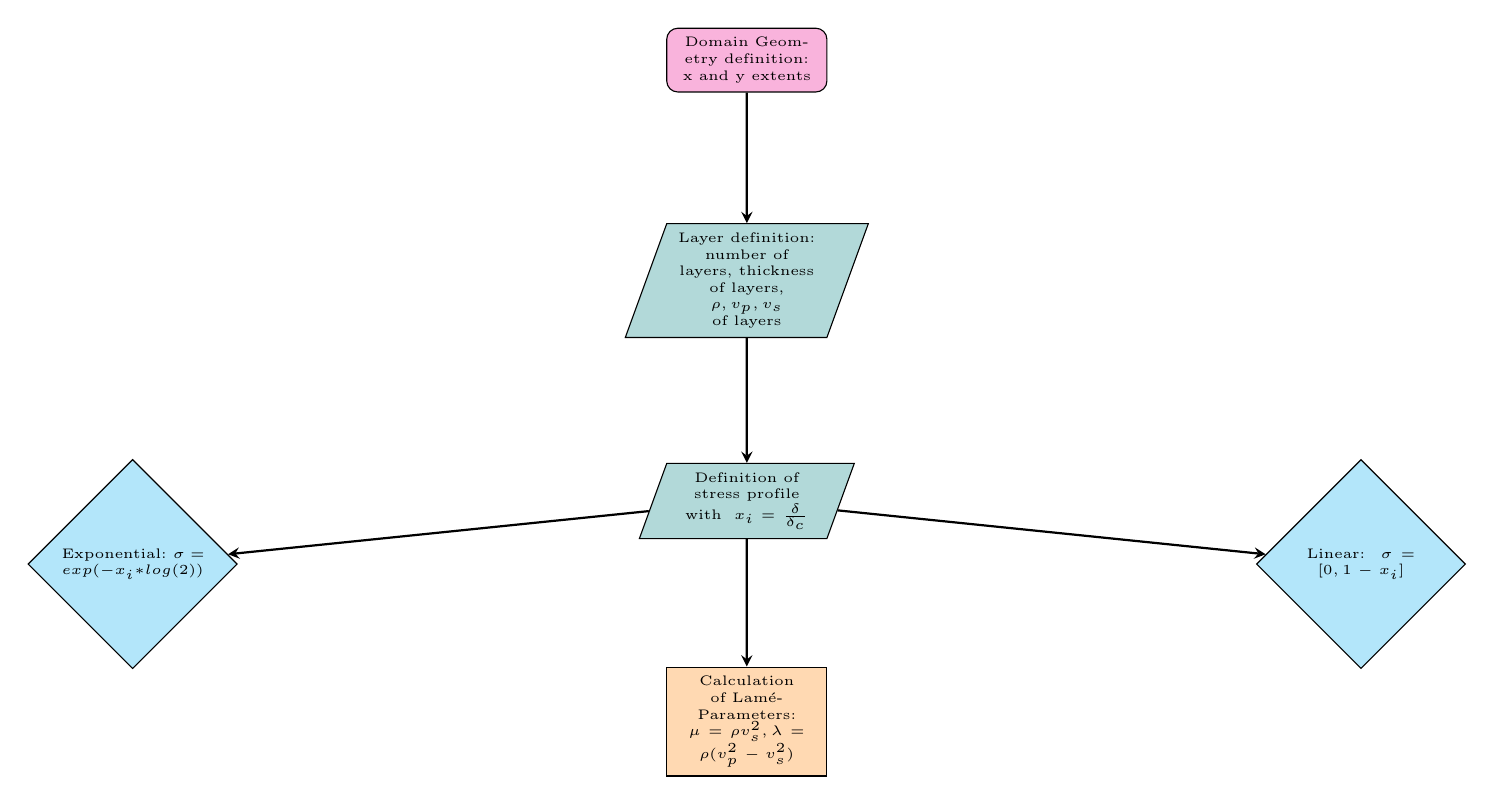
\begin{tikzpicture}[node distance=2.8cm]
  \centering
  \node (start) [startstop] {Domain Geometry definition: x and y extents};
  \node (in1) [io, below of=start] {Layer definition: number of layers, thickness of layers, $\ \rho, v_p, v_s$ of layers};
  \node (pro1) [io, below of = in1] {Definition of stress profile with $\  x_i = \frac{\delta}{\delta_c}$};
  \node (stress1) [decision, right of=pro1, xshift=5cm, yshift=-0.8cm] {Linear: $\  \sigma = [0, 1-x_i]$};
  \node (stress2) [decision, left of= pro1, xshift=-5cm, yshift=-0.8cm] {Exponential:$ \ \sigma = exp(-x_i * log(2))$ }; 
  \node (pro2) [process, below of=pro1] {Calculation of Lamé-Parameters: $\ \mu = \rho v_s^2, \lambda = \rho (v_p^2 -v_s^2)$};

  \draw [arrow] (start) -- (in1);
  \draw [arrow] (in1) -- (pro1);
  \draw [arrow] (pro1) -- (stress1);
  \draw [arrow] (pro1) -- (stress2);
  \draw [arrow] (pro1) -- (pro2);
\end{tikzpicture}

\subsubsection*{Part 2: Material Properties and Process Zone Calculation}
\begin{tikzpicture}[node distance=3.8cm]
  \centering
  % \node (pro2) [process] {Calculation of Lamé-Parameters: $\ \mu = \rho v_s^2, \lambda = \rho (v_p^2 -v_s^2)$};
  \node (pro3) [process, below of=pro2] {Calculation of Elastic modulus from Lamé-Parameters: $\ E = \mu * (3.0 * \lambda + 2.0 * \mu) / (\lambda + \mu)$};
  \node (pro4) [process, below of=pro3] {Calculating slip profile: array of zeros at every slip position, $\int_{0}^{1}(1-\sigma(\xi))d\xi$, where $\ \sigma(\xi)$ is the stress profile. The slip is distributed elliptically: $\ slip \propto \sqrt{4\xi (1-\xi)}$, where $\ \xi = \frac{x-x_{start}}{x_{end}-x_{start}}$};
  \node (pro5) [process, below of=pro4] {Calculating slip distance: distance between current position and crack tip is calculated, if in front of tip, the slip is 0. If the current position is behind the crack tip, then: $\ x_i = \frac{1 - \Delta x}{l_{cz}}$, where $\ l_{cz}$ is the cohesive zone length};
  \node (in2) [io, below of=pro5] {Normal and shear strengths and critical fracture energies measured by \cite{mahajanModelingInterfacialCrack2008} used to calculate critical separations: $\ \Delta n = 2*G_I$ / \sigma}; 
  \node (pro6) [process, below of=in2] {Calculating process zone lengths for shear and normal forces: $\  l_{ch} = E_{eff} * G_{IIc} / max(\tau_s^2, 1e-12), l_{cz} = \pi / 8.0 * l_{ch}$}; 
  \node (in3) [io, below of=pro6, yshift=-3cm] {Rupture speed calculation: minimum shear wave speed is adjusted for thickness and stiffness of interface according to the [0.5,2] interval of $\ \sqrt{\frac{E_{eff}}{10e6},\sqrt{thickness}}$. These corrections are the weighted, rupture velocity is calculated according to bounds described by \cite{trottetTransitionSubRayleighAnticrack2022}: between 0.25 and 0.6 vs for sub-Rayleigh, above 1.6 vs for supershear };

  % \draw [arrow] (pro2) -- (pro3);
  \draw [arrow] (pro3) -- (pro4);
  \draw [arrow] (pro4) -- (pro5);
  \draw [arrow] (pro5) -- (in2);
  \draw [arrow] (in2) -- (pro6);
  \draw [arrow] (pro6) -- (in3);
\end{tikzpicture}

\subsubsection*{Part 3: Rupture Propagation and Source Definition}
\begin{tikzpicture}[node distance=3.8cm]
  \centering
  % \node (in3) [io] {Rupture speed calculation: minimum shear wave speed is adjusted for thickness and stiffness of interface according to the [0.5,2] interval of $\ \sqrt{\frac{E_{eff}}{10e6},\sqrt{thickness}}$. These corrections are the weighted, rupture velocity is calculated according to bounds described by \cite{trottetTransitionSubRayleighAnticrack2022}: between 0.25 and 0.6 vs for sub-Rayleigh, above 1.6 vs for supershear };
  \node (pro7) [process, below of=in3] {Calculation of rise time (duration of slip) from cohesive zone length and rupture speed: $\ t = \frac{l_{cz}}{v_{rupture}} $}; 
  \node (in4) [io, below of=pro7] {Definition of crack zone length by defining start and end x position, spacing of sources, ratio between mode I and mode II}; 
  \node (pro8)[process, below of=in4]{Calculation of onest time (time where source at x position needs to fire): $\ t_{onest} = (x_i - x_0) / v_{rupture}$}; 
  \node (pro9) [process, below of=pro8] {Calculation of moment tensor source direction: $\ M0 = \mu * slip * \Delta x,  m_{xy} = mode_{mix} * M0, m_{yy} = -(1.0 - mode_{mix}) * M0, m_{xx} = 0.0$ }; 
  \node (pro10) [process, below of=pro9] {Appending all subfault slip distances, source directions and onset times to salvus project};
  \node (end) [startstop, below of=pro10] {Simualtion launch and plotting}; 

  \draw [arrow] (in3) -- (pro7);
  \draw [arrow] (pro7) -- (in4);
  \draw [arrow] (in4) -- (pro8);
  \draw [arrow] (pro8) -- (pro9);
  \draw [arrow] (pro9) -- (pro10);
  \draw [arrow] (pro10) -- (end);
\end{tikzpicture}



% \subsection{Crack Types Relevant for Avalanche Release}
%   \begin{itemize}
%     \item Anticracks: Cracks that close after opening \parencite{gaumeDynamicAnticrackPropagation2018}, in other words, this means that the weak layer collapses under loading, which leads to the opening of cracks in layers above because of the collapse \parencite{knightSuperheatedIceTrue1972}. This introduces frictional contact between the crack faces. 
%     \item Mode I: space is opened between the crack faces under tensile loading \parencite{heierliAnticracksNewTheory2003}.
%     \item Mode II: parallel shearing \parencite{heierliAnticracksNewTheory2003}.
%     \item Mode III: diagonal shearing \parencite{heierliAnticracksNewTheory2003}. (see figure in \cite{mahajanModelingInterfacialCrack2008} for clarifiction)
%   \end{itemize}

%   \subsection{Terminology according to \cite{ramosWorkingDynamicEarthquake2022}}
%   \begin{itemize}
%     \item Cohesive zone \Lambda : fundamenta length scale in rupture models where the fault strength decreases from static to dynamic level
%     \item Critical slip distance: slip needed for fault strength to drop from static level to dynamic level
%     \item Cracklike rupture: in such a model, the rise time is about equal to the total rupture duration: this means it takes the same amount of time for the slip to reach its highest value, as the time the whole fault rupture lasts
%     \item Dynamic fault strength: fault strength during the rupture: $\ \sigma_d = \sigma_n ^{eff} x \mu_{dynamic} $, which is the product of effective normal stress and the dynamic friction coefficient
%     \item Dynamic stress drop: difference in shear stress before and during earthquake (rupture)
%     \item Fracture energy: energy needed to grow a propagating crack
%     \item Slip: displacement at a given location on a fault
%     \item Stress drop: difference between static strength (strength before) and thedynamic strength (during rupture)
%     \item Static stress drop: difference in shear stress before and after, the average over the fault area is $ \ \Delta \sigma = \bar{\Delta \sigma_s} = \frac{1}{A} \int \Delta \sigma_s dA$, where $ \ \sigma_s$ is the static fault strength
%     \item Static afult strength: fault strength before movement: $ \ \sigma_s = \sigma_n ^{eff} x \mu_{static}$
%   \end{itemize}

%   \subsection{Other points from \cite{ramosWorkingDynamicEarthquake2022}}
%   \begin{itemize}
%     \item In mode II ruptures, two degrees of freedom lead to the generation of P- and SV-waves (vertically polarized shear wave)
%     \item Mode III can only generate SH-waves in homogenous media
%     \item Mode I represents tensile crack which is not usually important for dynamic rupture, but point-source models can account for fault opening by separating tensor into different components
%     \item Different modeling methods use different forms of eqations: FE and SE use weak form, PSE and FD use strong form. Weak form implicitly satisfies Neumann boundary conditions, which means that only Dirichlet need to be implemented. Meshes can also be more complex, because a lower oder derivative of the equations is used
%     \item During dynamic rupture, the cohesive zone width is a critical parameter, it can be estimated depending on the friction law used: for the linear slip-weakening friction law (frictional coefficient decreases linearly as slip propagates): $ \ \Lambda = \frac{C_1}{C_2} [\frac{GD_c}{\Delta \sigma_d}]^2[\frac{1}{1 + \frac{L_0^2}{L^2}}]$, where $ \ L_0$ is the critical half-crack length
%     \item Friction law describes how the friction evolves over time, this is an important choice
%     \item Slip weakening when slip is greater than dynamic friction coefficient
%     \item SLip strengthening when slip is smaller than static friction coefficient -> this can be used to model crac k arrest
%     \item No energy to grow crack when they are equal 
%     \item Velocity dependent frcition weakening law 
%   \end{itemize}

%   \subsection{Processes linked to crack propagation}
%   \begin{itemize}
%     \item Loading \& loading rate: initial loading which can trigger crack propagation. The propagation of cracks can be upslope from the loading point, which can mean that avalanches are triggered remotely \parencite{gaumeDynamicAnticrackPropagation2018} or propagation can be downslope, which means that the avalanche is triggered at the loading point \parencite{gaumeDynamicAnticrackPropagation2018}. Which direction the propagating cracks have, is influenced by model scale, as discussed by \cite{gaumeDynamicAnticrackPropagation2018}. Loading can be slow, for example by snow accumulation, or rapid, for example by a skier or an explosion. Slow loading can lead to sintering, which means that new bonds are formed between snow grains, which can strengthen the material and delay failure \parencite{mulakNumericalInvestigationMixedmode2019}. Rapid loading does not allow for sintering to occur, which means that there is still failure \parencite{mulakNumericalInvestigationMixedmode2019}.
%     \item Coupled criteria: There needs to be enough stress on the slab to exceed the weak layer strength (enough force for cracks to initiate because of failure), but also enough energy so that cracks can propagate. This means that two conditions need to be met for avalanche release. 
%     \item Snow Mechanical Properties: properties of the snowpack influence crack propagation. Slab bending in steep terrains for example can lead to supershear crack propagation \parencite{trottetTransitionSubRayleighAnticrack2022}. The weak layer thickness also has an influence on crack propagation \parencite{gaumeModelingCrackPropagation2015}. 
%     \item Strain softening: this means that less stress is required to have deformation, in other words, the material becomes weaker as it deforms. This is important because strain softening can lead to faster crack propagation, which could lead to faster slab breakoff. 
%   \end{itemize}


%   \subsection{Crack Areas}
%   \begin{itemize}
%     \item Crack tip: front of the crack, this is where the crack propagates
%     \item 
%   \end{itemize}

%   \subsection{Governing equations of crack propagation}
%   \begin{itemize}
%     \item Nucleation: Stress condition: $\ \sigma ≥ \sigma_c$, which means that the stress due to loading ($\ \sigma $) must exceed the weak layer strength ($\ \sigma_c $) over a certain distance \parencite{rosendahlModelingSnowSlab2020}. 
%     \item Energy criterion: $\ G ≥ G_c $: the energy available from the slab deformation (G) needs to be greater or equal than the fracture toughness of the weak layer, which means there needs to be enough energy for new cracks to form and to propagate \parencite{rosendahlModelingSnowSlab2020}.
%     \item Critical crack length: $ \ r_c = \Lambda \sqrt{\frac{2E'G_c}{\sigma^2}}$. E' is the slab elastic modulus, \sigma the applied stress. The critcial crack length is the length at which a crack becomes self-propagating and can lead to slab breakoff \parencite{gaumeModelingCrackPropagation2015}. 
%     \item Timoshenko beam representation: takes into account shear and rotational deformation of a beam, \cite{mahajanModelingInterfacialCrack2008} represent the snow slab as a Timoshenko beam. 
%     \item Slip and displacement: relative displacement between slab and weak layer \parencite{mahajanModelingInterfacialCrack2008}
%     \item Fracture energy: Energy required to create a crack is the area under the traction-separation curve \parencite{mahajanModelingInterfacialCrack2008}
%   \end{itemize}

% \subsection{Crack representation in past models}

% \subsubsection{\cite{burridgeAdmissibleSpeedsPlaneStrain1973}}
% \begin{itemize}
%   \item discusses different cases for crack propagation speed based on equations
%   \item Modeled a crack that propagates at a constant velocity from a point
%   \item Crack modeled has friction, but no cohesion, this means that the resistance which needs to be overcome is only from friction
%   \item For rayleigh-speed propagating cracks: a peak shear stress develops ahead of the crack tip 
%   \item Speed of the crack depends on static friction: if this is high, then crack propagates sub-Rayleigh
%   \item If static friction is lower, then the low stress peak at the front can exceed material strength before the crack arrives 
% \end{itemize}

% \subsubsection{\cite{andrewsRuptureVelocityPlane1976}}
% \begin{itemize}
%   \item Stress drops when slip starts: this is mathematically the same as motion
%   \item Material can only support a certain amount of stress: stress singularity satisfying fracture criterion (critical stress needed for fracture formation)
%   \item Elastic energy loss at the crack tip in previous media
%   \item Different friction law where friction at crack tip decreases linearly over critical slip distance
%   \item Mother daughter mechanism of cracks: crack nucleates at sub-rayleigh speed, stress peak grows at it accelerates toward rayleigh speed, stress peak nucleates a daughter crack, which moves at supershear speeds, eventually the daughter crack fuses with the mother crack again
% \end{itemize}

% \subsubsection{\cite{mcclungFractureMechanicalModels1981}}
% \begin{itemize}
%   \item linear elastic fracture mechanism: stress is singular at the crack tip --> only works if there is no deformation before crack propagation
%   \item Discusses a shear crack model: shear band \& slip deformations
%   \item Displacement of crack is related to stress applied
%   \item No friction on crack faces
%   \item End zone is the length where the stress drops from initial stress to the residual stress. This is observed because of strain softening: stress needed for same displacement is less with time
%   \item If crack length is about the same as the size of the zone where deformation is plastic, there is no propagation becaus ethe energy needed for propagation is too large and there is yielding instead of propagation of cracks
%   \item The propagation of cracks is dependent on the intensity factor of modes I and II stresses, initial and residual stress, the average slip in the end zone. Resulting from this is the propagation condition for the shear band.
%   \item The crack length might be many slab thicknesses large, this means that there is a relationship between slab thickness
%   \item Model focuses on large-scale deformations instead of microscale failure. These are independent of slab properties
%   \item Model represents crack propagation in weak layer (described as shear band) with initial loading, but no loading after initial loading
%   \item Shear band is described by contrast in material properties
%   \item Different shapes of weak layers discussed: band, but also elipsoidal inclusion with fixed location
%   \item For elipsoidal zone: stress is related to normal strain, weakened zone parameters, shear stress magnitude and axis ratio of elipsoidal weak zone
%   \item Incremental relationships describing yielding vs dilatancy (volume increase under loading), which can also be made slope-angle dependent
%   \item Plastic softening / hardening is 0 in a flat zone 
%   \item In this model, slope angle has no effect on critical moduli relations, but it's important for plastic deformation 
%   \item There can be localized shear band formation (new shear bands form in different locations) because deformation pattern can bifurcate 
%   \item The first fracture observed is a tension fracture whcih propagates across the slope because of stress propagation in the weak layer. The angle between the shear bed and the tension fracture is observed to be 90° ± 10° . 
%   \item Tension stresses cannot be formed before there is a shear band in this model (no stresses without a weak layer)
%   \item Stresses at different locations of shear band can be calculated
%   \item If distance needed for stress to drop from initial to residual is lower than one slab thickness, then the principal tension stress increases and concentrates -> again slab thickness dependency
%   \item If the propagation speed increases, the initial angle of propagation also increases
%   \item Shear disturbances need some anisotropy to propagate
%   \item Initial fracture location dependent on stress concentration due to topographic effects
%   \item Sequence of fractures: Initial shear failure first, the strain softeing, propagation of the shear disturbance, followed by tension fracture in the snow slab which is concentrated at the shear bed surface, loading drives disturbance further, which leads to flank fracturesa and lastly failure at the lower boundary of slab
%   \item Weak layer thickness has no effect in this model because deformation is mostly shear
% \end{itemize}

% \subsubsection{\cite{bazantFractureSizeEffect2019}}
% \begin{itemize}
%   \item Fracture mechanics determines material failure by energy criteria, sometimes in combination with strength criteria
%   \item Fracture theory considers failure to propagate through the medium rather than through the entire failure zone at the same time
%   \item Previously, fracture mechanics only applicable to homogenous britte materials (like glass, which is homogenous but still fails in a brittle manner)
%   \item This is a problem, because many materials, including snow, are heterogenous but still have brittle failure: this book focuses on concrete
%   \item Linear elastic failure mechanics based on the solution for stresses at the vertex of an ellipsoidal cavity: stress cannot be used as a criterion because at the crack tip, stress is infinite --> crack propagation if energy is available 
%   \item Energy which needs to be available is $ \ 2\gamma_s$, where $ \ \gamma_s$ is the specific surface energy of the elastic solid
%   \item Energy required for crack propagation is larger than specific surface energy, it was later defined as crack resistance -> can be described as a curve dependent on crack length
%   \item Fracture mechanics requires a certain energy to form crack: crack initiation energy 
%   \item Smeared cracking: does not take into account fracture mechanics, stress is a finite element limited by tensile stregth of material. after stress limit is reached, stress must decrease -> gradual release of stress as strain softening 
%   \item Two main types of failure: plastic and brittle. In plastic failure, structure develops a single degree of failure mechanism, this means that failure proceeds simulatiously at different points in the material. Plastic failure when the yield plateau is long on the load-deflection diagram: large area where deformation is plastic. If such a plateau does not exist, there is brittle failure
% \end{itemize}

% \subsubsection{\cite{mahajanModelingInterfacialCrack2008}}
% \begin{itemize}
%   \item Desrcibe a cohesvie zone model (CZM)
%   \item Focuses primarily on mode II fractures
%   \item Model is defined by 4 physical properties of snow, which were determined by experments: tenisle and shear stregth, normal and shear fracture energy
%   \item Here, a narrow-band fracture can exist ahead of the crack tip. This is important because the fracture process is distributed over a finite zone, so the crack can be described by a traction-displacement relation across the band rather than by a single sharp tip.
%   \item In the CZM, there is softening to force relation: the opening of the cracks and peak stresses are contained under the force-displacement curve -> softening law 
%   \item Cracks occur, when the peak stress occurs and traction is reduced to zero
%   \item Material characterized on both sides of narrow-band frcature: relation between traction and displacement across the band 
%   \item Initial crack needed for further failure in model 
%   \item Mass matrix as a combination of internal and external forces 
%   \item Initial forces contribute to cohesive element tracttions, external forces to body forces and external loads
%   \item Stress opening is a potential function with tangential and normal components, which have characteristic normal and shear separation distances
%   \item Traction decreases as cohesive surfaces separate, it approaches 0 as the separation increases
%   \item Strain softening occurs in this model when the separation distances corresponding to cohesive normal and tangential strength have been exceeded
% \end{itemize}



\section{\textbf{Notes}}

- Look into wave modes (flexural and other mode)



% \section{Synthesis}
% The papers discussed can be divided into two methods utilized to model snow processes. Understanding how snow can be modeled accurately and efficiently is very relevant for the thesis, because a large part of the thesis will be modeling DAS data of avalanches in snow. This is why it is important to understand the different methods used to model snow and their advantages and disadvantages as well as the physical processes underlying these models.
% A majority of the papers discussed below utilize the discrete element method described by \cite{cundallDiscreteNumericalModel1979}. In this method, the interaction between individual grains is modeled by calculating the forces and the resulting displacements on the grains \parencite{cundallDiscreteNumericalModel1979}. This method is both used to describe snow failure as well as crack propagation in snow, for example \cite{gaumeModelingCrackPropagation2015} model crack propagation in a weak snow layer using discrete elements. This modeling method is accurate in modeling snow processes, but as described by \cite{bobillierMicromechanicalModelingSnow2020}, it models snow on the grain scale, which is computationally expensive when modeling snow on the slope scale. \cite{bobillierMicromechanicalModelingSnow2020} developed a model on the particle scale, which is still accurate at a higher computational efficiency.
% Another method used by some papers is the material point method. This method discretizes the material into a set of material points, which are used to calculate the deformation and stress of the material \parencite{gaumeDynamicAnticrackPropagation2018}, the time dependent equations can only be solved by using an Eulerian background mesh. This method is used by multiple papers, to model crack propagation, for example \cite{gaumeDynamicAnticrackPropagation2018} use this method to model crack propagation in snow.
% The MPM method is advantageous over the discrete element method because it is more computationally efficient, which means that it can be used to model larger scale processes such as slope scale avalanches, whereas the discrete element method is more accurate but computationally expensive, which means that it is more suitable for modeling smaller scale processes such as crack propagation in a weak layer. In MPM, contacts are modeled in the background grid, whereas in DEM they are modeled individually and every time a contact is made or broken, the stiffnesses need to be recalculated. The MPM method also allows for modeling of strain softening, more easily, this is important when modeling snow processes. Modeling strain softening using discrete element methods is possible, but more difficult because elements need to be removed manually to account for the cracks closing, whereas in the MPM method, strain softening can be modeled by a yield surface with varying pressure, which allows for strain softening even at macroscopic uniaxial compression \parencite{gaumeDynamicAnticrackPropagation2018}.
% Snow can also be modeled by physical models for snowpacks, such as SNOWPACK described by \cite{barteltPhysicalSNOWPACKModel2002} or CROCUS described by \cite{brunNumericalModelSimulate1992}. These models implement processes such as snow metamorphism and settling of snow, which are important to understand where weak layers form. Both models developed by \cite{brunNumericalModelSimulate1992} and \cite{barteltPhysicalSNOWPACKModel2002} account for changes in microstructure of snow and the effects of snow layering and temperature gradient changes. Understanding what effect these processes have on snow structure is important to understand where avalanches will likely form, but it is not necessary to model these processes in the thesis, because the focus is not on snowpack evolution.
% \cite{mulakNumericalInvestigationMixedmode2019} show that sintering, which means the formation of new bonds between snow grains, is an important process to consider when modeling snow failure, because it can increase the strength of the material and delay failure. This is important to consider for the thesis because it can mean that there is a large time between loading and failure, which can influence whether cracks are observed in DAS data and how long it takes between initial cracking and avalanche release. However, \cite{mulakNumericalInvestigationMixedmode2019} also show that if there is rapid loading, sintering is too slow to prevent failure, which means that in cases of rapid loading, sintering does not need to be considered. This is relevant for the thesis because in cases of rapid loading, such as a skier triggering an avalanche, sintering does not need to be considered, whereas in cases of slow loading, such as a large accumulation of snow, sintering needs to be considered. Such processes are neglected in the model developed by \cite{rosendahlModelingSnowSlab2020} as well as the model by \cite{gaumeInvestigatingReleaseFlow2019}, who develop models only for the fast-loading case. Understanding the effect of sintering is important to represent snow processes accurately in the thesis: does the loading occur over large times (by snow itself) or is it a rapid loading event (skier or explosion). \textcolor{magenta}{ \begin{itemize}
% \item  Could different models be made depending on loading rate to compare DAS data?
% \item Could DAS data look different for rapid and slow loading? 
% \end{itemize}
% }
% Multiple papers show that after loading, there are different stages of deformation of snow. \cite{gaumeDynamicAnticrackPropagation2018} showed that snow responds to loading by an elastic regime, a drop in pressure and shear stress, volumetric collapse of the weak layer and lastly dense packing. \textcolor{magenta}{do these stages show up individually in DAS data or are they one event?}. \cite{bergfeldSignaturesSubRayleighSupershear2025} also discuss different deformations, but mainly related to the location in the snowpack. At the lower areas, deformation is because of slab bending caused by weak layer collapse, whereas higher in the snowpack, deformation is because of tension of the slab.
% Several papers also highlight that not all cracks trigger release: a crack must reach a critical length before a slab can detach \parencite{gaumeSnowFractureRelation2017a}, and the required length is sensitive to slab stiffness, slab thickness, weak-layer thickness, slab density, and slope angle. The weaker the snowpack, the lesser the crack length needed for failure. Related to this,  crack growth can occur in different modes: mode I (opening) versus mode II (shear), and mixed-mode loading changes the critical stress for propagation \parencite{rosendahlModelingSnowSlab2020}. These concepts are important for DAS interpretation because only cracks that approach (or exceed) their critical length are likely to produce a large enough deformation signal and to lead to avalanche release, whether this happens is related to snow parameters. 

% All the papers discussed below show that avalanches are triggered by initial loading, which causes failure in a weak layer, which then propagates through the snowpack. Understanding how the failure or cracks propagate through the weak layer and how this is modeled is important to model DAS data because the type of avalanche, the time between loading and release and whether there is an avalanche at all depends on the type of failure and crack propagation. Multiple papers discuss the type of crack propagation in snow, for example anticrack propagation, as well as the different processes influencing crack propagation.
% \cite{gaumeModelingCrackPropagation2015} show that the type of crack propagation in snow is influenced by the slope angle, the elastic modulus of the slab and the elastic modulus of the weak layer. If young's modulus of the slab is high, the density of the snow is high or the weak layer thickness is high, cracks propagate less far because failure occurs faster, which means that there is less time for cracks to propagate. If the tensile strength of the slab is high, crack propagation speed is higher, because the slab can sustain more stress before failure occurs, which means that there is more time for cracks to propagate. If the weak layer is very weak, crack propagation speed is also very low, because failure occurs before cracks have propagated. Direct failure also occurs when the slab is very soft \parencite{bobillierNumericalInvestigationCrack2024}. Furthermore, \cite{gaumeSnowFractureRelation2017a} show that the type of crack propagation is influenced by the slope angle, on flatter terrain, the bending of the slab is limited by the collapse depth, which leads to a constant speed of crack propagation, whereas in inclined terrains, slab tension can increase, which also leads to crack propagation speeds to increase \parencite{trottetTransitionSubRayleighAnticrack2022}.  \cite{bobillierNumericalInvestigationCrack2024} also show that slope angle is important for the crack propagation speed. At high slope angles, \cite{bobillierNumericalInvestigationCrack2024} observe crack propagation speeds higher than the shear velocity in the material (supershear), whereas at lower slope angles, the propagation speed of cracks is lower (sub-Rayleigh). As described by \cite{trottetTransitionSubRayleighAnticrack2022}, the faster cracks propagate, the faster the slab breakoff will occur, which means there is less time between the initial cracking and the release of the avalanche.
% \cite{bergfeldSignaturesSubRayleighSupershear2025} make the link between shear crack propagation and anticrack propagation. In their simulations and lab experiments, \cite{bergfeldSignaturesSubRayleighSupershear2025} show that early stages of crack propagation are anticrack-dominated, while at later stages, shear cracks occur. Again, if the system reaches supershear propagation is dependent on multiple factors, as previously mentioned. The size of the release area observed by \cite{bergfeldSignaturesSubRayleighSupershear2025} is dependent on crack arrest, which is dependent on the propagation regime. Supershear speeds only show crack arrests because of topography, which leads to larger release areas \parencite{bergfeldSignaturesSubRayleighSupershear2025}. The relationship between crack propagation regime and release area is important because it can help making more accurate risk assessments based on DAS data: if the crack propagation is supershear, there is a higher risk of a large release area, which means that the avalanche can have higher volume.
% Multiple papers also mentioned that the propagation direction crack propagation is dependent on the scale of the simulation. Understanding in which direction cracks propagate is not only important to understand where the slab will break off, it is also important to understand where in relation to the DAS cable the breakoff event can be observed. \cite{gaumeInvestigatingReleaseFlow2019} show that in small scale simulations, cracks propagate upslope, whereas in larger scale simulations, cracks propagate downslope. This is explained by \cite{trottetTransitionSubRayleighAnticrack2022} by the fact that in small scale simulations, the bending of the slab is limited by the collapse depth, which leads to a constant speed of crack propagation, whereas in inclined terrains, slab tension can increase, which also leads to crack propagation speeds to increase \parencite{trottetTransitionSubRayleighAnticrack2022}.





% \section{Avalanche \& Snow Modeling}

% \subsection{Micromechanical modeling of snow failure \parencite{bobillierMicromechanicalModelingSnow2020}}
% \textbf{Main Question of article:} Can crack and mechanical behavior be represented in a computationally efficient model on the slope scale?\par

% \textbf{Why this is relevant for the thesis:} Understanding how to model snow and snow mechanical behavior is important to model DAS data in snow accurately.\par
% Models previous to \cite{bobillierMicromechanicalModelingSnow2020} represent crack behavior accurately, but on the grain scale, which is very computationally inefficient when simulating slope-scale processes. \cite{bobillierMicromechanicalModelingSnow2020} used a discrete element model on the particle scale, which acts as a mesoscale between the grain level and the snow sample scale. The model developed agrees with data from cold-lab experiments. The model used is a three layer model with a rigid basal layer, a weak layer and a slab layer \parencite{bobillierMicromechanicalModelingSnow2020}. Under tensional regimes, \cite{bobillierMicromechanicalModelingSnow2020} observed elastic-brittle failure in snow, whereas the weak layer, under mixed loading, showed four distinct deformation stages. The stages can be described as elastic deformation, strain softening which happens at the same time as brittle crushing of particles, followed by shear displacement \parencite{bobillierMicromechanicalModelingSnow2020}. 


% \subsection{Numerical investigation of the mixed-mode failure of snow \parencite{mulakNumericalInvestigationMixedmode2019}}
% \textbf{Main Question of article:} What influence do different loading angles and rates have on failure criteria of snow layers and what effect does sintering have on this?\par

% \textbf{Why this is relevant for the thesis:} Understanding the effect of loading rates, loading angles and failure modes is very important to understand effects seen in DAS data: this influences the type of avalanche, the time between loading and release and whether there is an avalanche at all\par
% Snow material failure resulting in avalanches occurs on the individual bond scale, simultaneous shear and compressive loading further increases the complexity \parencite{mulakNumericalInvestigationMixedmode2019}. Understanding which loading angles and rates lead to which types of failure is of importance in understanding DAS data of avalanche release, because as \cite{mulakNumericalInvestigationMixedmode2019} show, these processes are quite complex. Sintering is an important process in understanding material failure, because broken bonds can be reformed, which can even increase the strength of material. \cite{mulakNumericalInvestigationMixedmode2019} state that if there is high stress, compression of the material increases, which leads to an increase in strength of the material and the failure is delayed. This has relevance for the thesis because there can be a large amount of time between the loading and the actual material failure. If there is rapid loading on the other hand, sintering is too slow and there is still failure \parencite{mulakNumericalInvestigationMixedmode2019}. Sintering in the avalanche case would occur if there is a large accumulation of snow and a slow increase in compressive load \parencite{mulakNumericalInvestigationMixedmode2019}. \textcolor{magenta}{Could the DAS data look different for rapid loading and slow loading because the stresses are different?}
% \cite{mulakNumericalInvestigationMixedmode2019} implemented a discrete element model where different failure conditions are investigated at loading angles between 0° and 180°. Failure is defined by an increase in average velocity of the slab (meaning the slab would slide) or an increase in maximum value of the stress \parencite{mulakNumericalInvestigationMixedmode2019}. \cite{mulakNumericalInvestigationMixedmode2019} implemented sintering in their model by the creation of new bonds in the discrete element structure. For simulations with no sintering, at low loading angles, there is a decrease in cohesive bonds, which further increases with higher loading angles \parencite{mulakNumericalInvestigationMixedmode2019}. This means that at low loading angles, the number of broken bonds required for material failure is much larger, as stated by \cite{mulakNumericalInvestigationMixedmode2019}. At higher loading angles, the total strength of the weak layer decreases, which means that the shear stress is dependent on loading angle \parencite{mulakNumericalInvestigationMixedmode2019}. Where sintering was implemented by \cite{mulakNumericalInvestigationMixedmode2019}, the results are almost the same as in the case without sintering. The number of broken bonds needed for failure is larger however, because new bonds can form, and the strength decreases more if the loading angle increases \parencite{mulakNumericalInvestigationMixedmode2019}. \cite{mulakNumericalInvestigationMixedmode2019} show that sintering is most important in compression-dominant modes at low loading angles. If sintering times are low, the failure of material occurs faster than the formation of new bonds, which means that the results without sintering are the same as the ones without sintering \parencite{mulakNumericalInvestigationMixedmode2019}. All simulation data show good agreement with lab data. Overall, \cite{mulakNumericalInvestigationMixedmode2019} also show that shear strength of a material is more crucial in material failure compared to compressive strength, because shear strength is often lower. This means that the shear load is more likely to cause failure as opposed to the compressive load \parencite{mulakNumericalInvestigationMixedmode2019}. The models developed by \cite{mulakNumericalInvestigationMixedmode2019} are only 2D, which is a limitation because porosity is limited, this limits strain softening and possible collapses of weak layers.



% \subsection{A physical SNOWPACK model for the Swiss avalanche warning: Part I: numerical model \parencite{barteltPhysicalSNOWPACKModel2002}}
% \textbf{Main Question of article:} How can the snowpack and its governing equations be modeled accurately but as simple as possible?\par

% \textbf{Why this is relevant for the thesis:} Modeling snowpack evolution and structure is important to forecast avalanches (where are avalanches likely to form), but also to understand avalanche dynamics (in which layers do avalanches form)\par
% \cite{barteltPhysicalSNOWPACKModel2002} describe that numerical modeling of the snowpack is important for avalanche prediction. The snowpack-model developed solves the partially governing equations using finite-element methods \parencite{barteltPhysicalSNOWPACKModel2002}. Understanding snowpack evolution and avalanche formation is also relevant for the thesis because the crack propagation which is modelled in the thesis depends on snow properties. According to \cite{barteltPhysicalSNOWPACKModel2002}, most avalanches occur during or after periods of intense snowfall. Snow settling gives an insight on mechanical stability of snow, which is also important to understand crack propagation: in stable layers cracks probably do not propagate as well as in layers which already have some instabilities. The microstructure and the layering of snow also needs to be modeled to detect discontinuities or layer boundaries, which is important to assess stability of layers \parencite{barteltPhysicalSNOWPACKModel2002}. \cite{barteltPhysicalSNOWPACKModel2002} also model the influence of solar radiation and warm winds on the energy exchange, the melting of snow and the subsequent transport of meltwater is important to understand the release of wet snow avalanches.
% Existing snowpack models such as CROCUS rely on Truesdell's equation for mixture and postulate conservation of ice, water, water vapor and air of the snowpack, these models are simplified \parencite{barteltPhysicalSNOWPACKModel2002}. This means that the existing models for example do not describe settling of the snowpack, they assume the snowpack to be dry or the absence of snow metamorphism, which does not depict the reality of the snowpack accurately \parencite{barteltPhysicalSNOWPACKModel2002}. An accurate and physical model of the snowpack is important for the thesis because modelled data should be comparable to field data measured by the DAS cable. This would not be the case if simplifications are made in the simulation of crack propagation in snow, the simulated data would look different from the measured data. The novel SNOWPACK model described by \cite{barteltPhysicalSNOWPACKModel2002} uses three constituents (ice, water and moist air) to describe the snow. These three all have the same temperature, which is the snow bulk temperature measured in meteorological observations, assume all meltwater processes to be energy and mass conserving and assume that the weight of the snowpack is carried by a single ice lattice \parencite{barteltPhysicalSNOWPACKModel2002}.
% \cite{barteltPhysicalSNOWPACKModel2002} use four governing equations to describe the snowpack: the energy transfer equation at the surface (conservation of mass of vapor and water and the bulk temperature), because all of the snow constituents have the same temperature, a momentum equation for settling of the snow because the weight of the snow is carried by a single ice lattice: The conservation of mass of ice is not considered because the numerical solution of the displacement is continuous because of the Lagrangian coordinate system. Any change in the snow load results in a change of the stress state of the settlement equation. Snow cannot be assumed to be a plastic material because deformations caused by loading are irreversible, understanding this is important for crack formation and propagation. \cite{barteltPhysicalSNOWPACKModel2002} describe a microstructure-based viscosity formulation, plasticity theory is not applicable because of time-dependent yield surfaces and a directionality of plastic flow which is defined in relation to the yield surface. The initial conditions of the snowpack such as snow height are taken from meteorological data, the energy exchange at the surface is the most important boundary condition \parencite{barteltPhysicalSNOWPACKModel2002}. Neumann boundary conditions are used if the temperature at the surface is close to the melting temperature, if the temperature is well below the melting temperature, Dirichlet boundary conditions are used \parencite{barteltPhysicalSNOWPACKModel2002}.
% The melting and refreezing processes in the snowpack are essential in modelling snow structure changes, which have an effect on DAS signal propagation as well as avalanche formation. \cite{barteltPhysicalSNOWPACKModel2002} model these by the numerical heat transfer solution. Because the snow temperature is assumed to be constant 0°C, if the heat transfer solution is greater than 0°C, the excess energy is assumed to be used for melting, if the heat transfer is smaller than 0°C, the energy is assumed to be used for refreezing \parencite{barteltPhysicalSNOWPACKModel2002}. \cite{barteltPhysicalSNOWPACKModel2002} used the snow structure measurements of winter 1999, which was a winter with numerous avalanches, to verify the SNOWPACK model developed.  Generally, there is good agreement between the measured and modelled data, which means that the model is physical, with some exceptions \parencite{barteltPhysicalSNOWPACKModel2002}. If the calculated snow height is different from the measured snow height, the model corrects this by adding elements to the finite element grid in case the calculated height is too low, or removing elements if snow height is overestimated \parencite{barteltPhysicalSNOWPACKModel2002}. This leads to mistakes if the snowpack settles quickly: if there is quick settlement, snow height decreases quickly because of densification, the model would remove elements at the surface without accounting for densification of the snow at the bottom \parencite{barteltPhysicalSNOWPACKModel2002}. Snow density and snow settlement have strong effects on heat conductivity of snow, \cite{barteltPhysicalSNOWPACKModel2002} mention that errors in either of these fields have strong effect on the entire simulation.
%  The SNOWPACK model developed by \cite{barteltPhysicalSNOWPACKModel2002} includes modeling of the microstructure of snow as well as density discontinuities, which represent layer boundaries, which is important to understand snow structure as well as crack propagation related to avalanches. The multicomponent description developed allows for representation of mass and energy conservation \parencite{barteltPhysicalSNOWPACKModel2002}, which can be used to assess snow metamorphism related to temperature and moisture, but also to determine where wet snow avalanches form due to the presence of water. \cite{barteltPhysicalSNOWPACKModel2002} describe the volumetric deformation of fresh snow by large strain description, the thermal boundary conditions which need to be used can be determined by meteorological data. These data can also be used to determine if there is melting or refreezing of snow, which again is important for snow structure and stability. The laws for heat conductivity and viscosity related to microstructure show the relations between densification of snow and heat transfer \parencite{barteltPhysicalSNOWPACKModel2002}. 

% \subsection{A numerical model to simulate snow-cover stratigraphy for operational avalanche forecasting \parencite{brunNumericalModelSimulate1992}}
% \textbf{Main Question of article:} How do snow conditions such as temperature gradient and water content influence snow metamorphism and how can this be implemented in the CROCUS-snowpack model?\par

% \textbf{Why this is relevant for the thesis:} Snow metamorphism changes grain properties, which is important for the formation of weak layers which can trigger avalanche release, but also overall stability of the snowpack. Furthermore, layers of different grain properties will depict DAS signals differently.\par
% When a snowpack is subjected to a change, like a change in temperature or pressure conditions, the snow grains change \parencite{brunNumericalModelSimulate1992}. Snow metamorphism changes the grain sizes and shapes, which changes mechanical stability of the snow \parencite{brunNumericalModelSimulate1992}. This is relevant for avalanche modelling because certain types of snow metamorphism can weaken layers in snow, such layers can act as failure planes and make release of avalanches easier. Snow metamorphism is affected by the water content of the snow, the capillary pressure of the water between the snow grains, the radius of curvature of the grains (shape), as well as the temperature gradient \parencite{brunNumericalModelSimulate1992}.
% \cite{brunNumericalModelSimulate1992} describes the main limitation of past metamorphism models as assuming the snowpack to have homogeneous shapes and sizes, which are often spherical or simplified geometric shapes, this does not represent snow accurately however, especially fresh snow is very heterogeneous. \cite{brunNumericalModelSimulate1992} conducted experiments for different snow types and conditions to determine new equations to describe metamorphism. These experiments showed that the rate and type of metamorphism does not depend on crystal type but rather on the temperature gradient \parencite{brunNumericalModelSimulate1992}. A gradient below 5°C/m results in rounded crystals, a gradient above 5°C/m results in faceted crystals, which transform to depth hoar, if a gradient of more than 15°C/m is applied \parencite{brunNumericalModelSimulate1992}. This is relevant for avalanche modelling, because it is critical to understand how snow grains evolve to assess their stability, which can be used to determine where weak layers will form. These experiments were conducted for dry and wet snow conditions.
% \cite{brunNumericalModelSimulate1992} describe a new description of snow, which takes into account the dendricity, sphericity and size of the grains. When snow falls, new layers with different properties are added to the snowpack \parencite{brunNumericalModelSimulate1992}. Simulating these different layers is again important to assess the stability as well as interactions of the different layers. \cite{brunNumericalModelSimulate1992} combined the observations made in the laboratory with the CROCUS snowpack model to simulate these different layers based on meteorological observations. Using MEPRA (a system for avalanche risk forecasting), the shear stress of the different layers was estimated at a 45° angle. This is important for avalanche forecasting, because the strength of different layers can be assessed and it can be determined under which stress the layers fail. 

% \subsection{A discrete numerical model for granular assemblies \parencite{cundallDiscreteNumericalModel1979}}
% \textbf{Main Question of article:} How can the forces and the resulting displacements be modeled in a granular medium?\par

% \textbf{Why this is relevant for the thesis:} Snow consists of grains, forces at the surface such as mechanical loading can cause displacement of the individual grains. If this happens at a very large scale, it is an avalanche.\par
% The distinct element method described by \cite{cundallDiscreteNumericalModel1979} is a numerical modeling method to model the mechanical behavior of a material composed of disks \& spheres. This is relevant to the thesis because snow is composed of individual snow grains, which interact with each other at their contacts, all the grains together form the snow pack. It is important to model the behavior and displacement of the grains to model avalanche dynamics because avalanches form through loading or failure in a weak layer, which then propagates through the entire snowpack \parencite{gaumeSnowFractureRelation2017a}.
%  Since a snowpack is a medium composed by individual snow grains, which are not entirely compacted (contain air between the grains) and interact with each other at grain contacts,  the medium described by \cite{cundallDiscreteNumericalModel1979} represents snow well. It is a granular medium composed of distinct particles, which interact with each other at their contacts and form a porous medium \parencite{cundallDiscreteNumericalModel1979}. The loading and unloading of such materials is complex and stresses cannot be measured easily because of the interactions of different grains \parencite{cundallDiscreteNumericalModel1979}.
% The distinct element method can model particles of any shape \parencite{cundallDiscreteNumericalModel1979}, which is important for snow modelling because the snow grains are not always spherical. \cite{cundallDiscreteNumericalModel1979} model the transient interaction of particles by calculating the contact forces and displacements of the stressed discs (particles) caused by disturbances at the boundaries. In the avalanche case discussed in the thesis, the disturbance is represented by loading of the surface, which can be caused by a skier, which causes failure in a weak layer, or cracking in the snowpack. This results in stress propagation through the snowpack, which results in displacement of the particles, which is the avalanche motion. The resultant forces on the disks are calculated only by the discs which are in direct contact (all the disks that touch one disk cause its resultant force) \parencite{cundallDiscreteNumericalModel1979}. \cite{cundallDiscreteNumericalModel1979} describe a model only for dry materials, this means this is only applicable for dry snow avalanches which contain no water between the snow grains.
% Numerical modelling, such as described by \cite{cundallDiscreteNumericalModel1979} is advantageous over lab tests and experiments because it is less time consuming and any data can be accessed at any stage, which means that parameters such as loading, particle size, and properties such as stiffness and shape can be changed at any stage. In the avalanche case, this means that simulations can be run for different snow properties and loading scenarios, for example a simulation for older, more compacted snow can be run as well as a simulation for fresh snow. The numerical model for spheres is based on methods described by Serrano and Rodriguez-Ortiz (1973, I CANNOT FIND THIS PAPER ONLINE). The forces at the interfaces between the spheres are calculated by incremental displacements of the centers of particles, where shape changes of the individual particles are negligible \parencite{cundallDiscreteNumericalModel1979}. \textcolor{magenta}{How can the center of the grain be determined if the grain has an irregular shape?} The matrix representing contact stiffness between the grains described by \cite{cundallDiscreteNumericalModel1979} needs to be recalculated whenever a new contact is made or broken, meaning when there is a crack in the snowpack or when new contacts between snow grains are made. The calculations of forces are based on Newton's 2nd law, which describes the movement of a particle as the result of the forces acting on it. The deformation is neglected because the deformation of individual particles is small compared to the deformation of the medium as a whole \parencite{cundallDiscreteNumericalModel1979}. This means that the deformation of the individual snow grains is small compared to the deformation of the entire snowpack which represents the avalanche movement. \textcolor{magenta}{What about the fusing / compaction of grains which changes snow properties?} The relative displacement of a particle is calculated by the sum of the force increments acting on it, particles can also overlap, in this case the contact forces and the interaction forces also need to be calculated \parencite{cundallDiscreteNumericalModel1979}. The location of the rigid boundaries (walls) described by \cite{cundallDiscreteNumericalModel1979} needs to be specified before modelling. This could be a possible limitation for the avalanche case because there is only one rigid "wall" which is the interface of snow and the rock below it. 



% \section{Crack Propagation}

% \subsection{Signatures of the sub-Rayleigh to supershear fracture transition in snow avalanche experiments \parencite{bergfeldSignaturesSubRayleighSupershear2025}}
% \textbf{Main Question of article:} Can supershear crack propagation be observed in snow avalanche field experiments and are there different stages of crack propagation?\par

% \textbf{Why this is relevant for the thesis:} Possible different stages of crack propagation speeds and their transitions are important for DAS data interpretation so that accurate risk assessments can be made.\par
% Previous to \cite{bergfeldSignaturesSubRayleighSupershear2025}, supershear fractures in snow have been observed in many numerical models, but never in slope experiments. \cite{bergfeldSignaturesSubRayleighSupershear2025} conducted controlled experiments on a snow-covered slope and did optical tracking of cracks, they also used MPM modeling to validate the slope experiments.
% Both the experiments and the numerical models showed that there are different stages in crack propagation \parencite{bergfeldSignaturesSubRayleighSupershear2025}. Understanding the different stages of crack propagation speeds and what causes the transitions between them is important to make accurate risk assessments based on DAS data: do cracks propagate slowly which causes a slow breakoff of the slab or is the propagation supershear? The different stages of crack propagation observed by \cite{bergfeldSignaturesSubRayleighSupershear2025} correspond with different locations in the snow: at the lower end of the snowpack, the deformation was dominated by slab bending induced by weak-layer collapse, whereas at the higher end, the deformation was dominated by slab tension which was induced by the shear failure of the weak layer \parencite{bergfeldSignaturesSubRayleighSupershear2025}. The results shown by \cite{bergfeldSignaturesSubRayleighSupershear2025} show that anticrack propagation dominates the early stage of crack propagation, but after a certain propagation distance, shear-driven fractures occur, especially on steeper slopes. This means that crack propagation leading to avalanches is a combination of both anticrack and shear fractures \parencite{bergfeldSignaturesSubRayleighSupershear2025}.
% Furthermore, in supershear crack propagation in the simulations by \cite{bergfeldSignaturesSubRayleighSupershear2025}, crack propagation was not arrested by slab fractures. This means that the release areas are much larger, because there is more extensive fracturing and faster propagation \parencite{bergfeldSignaturesSubRayleighSupershear2025}. For sub-Rayleigh crack propagation, \cite{bergfeldSignaturesSubRayleighSupershear2025} observed crack arrest if there are existing slab fractures, which leads to smaller release areas. This is critical for the thesis because if crack propagation is slower, this means that the avalanche released is likely smaller. \textcolor{magenta}{This is only a valid conclusion if the individual cracks can be observed}

% \subsection{Numerical investigation of crack propagation regimes in snow fracture experiments \parencite{bobillierNumericalInvestigationCrack2024}}
% \textbf{Main Question of article:} How do different snow mechanical parameters influence crack propagation speed?\par

% \textbf{Why this is relevant for the thesis:} Understanding the influence between crack propagation speed and snow parameters is important to understand when cracks can be observed in DAS data if at all and how long it takes between initial cracking and avalanche release.\par
% In previous models of crack propagation in snow, the mechanical properties of snow were not considered \parencite{bobillierNumericalInvestigationCrack2024}. A 3D discrete element model was developed by \cite{bobillierNumericalInvestigationCrack2024} to investigate the mechanical properties of snow of crack propagation in a PST, this was done at different slope angles. \cite{bobillierNumericalInvestigationCrack2024} assumed in their model that sintering and other time-dependent effects have no influence on crack propagation. A three-layered model consisting of a rigid bottom layer, a weak layer resembling depth hoar, as well as a dense slab layer was implemented \parencite{bobillierNumericalInvestigationCrack2024}. This type of model can possibly also be considered in the thesis. Understanding how different mechanical parameters affect crack propagation is relevant for the thesis because it influences if cracks can be observed in the DAS data at all, and if they are, how long it takes between initial cracking and slab breakoff, which is dependent on crack propagation speed.
% During the propagation saw test, the crack propagation speed reaches steady state, the numerical simulation results by \cite{bobillierNumericalInvestigationCrack2024} show that this is largely dependent on slope angle. At slope angles lower than 30°, the steady-state propagation speed is sub-Rayleigh, if the slope angle is greater or equal to 30°, the steady-state speed is larger than the shear wave speed, so supershear \parencite{bobillierNumericalInvestigationCrack2024}. It also depends on the slope angle how long it takes to reach this steady-state speed \parencite{bobillierNumericalInvestigationCrack2024}.
% \cite{bobillierNumericalInvestigationCrack2024} show that the higher the slab elastic modulus, the lower the normalized crack propagation speed, this is the opposite for weak layer elastic modulus: the higher the weak layer elastic modulus, the higher the crack propagation speed. If the weak layer is very weak, crack propagation speed is also very low, \cite{bobillierNumericalInvestigationCrack2024} explain this by failure occurring before cracks have propagated. Direct failure also occurs when the slab is very soft \parencite{bobillierNumericalInvestigationCrack2024}. These considerations are important for the thesis because it can mean that cracking might not be observed before the slab break off, or if the system is too stable, cracking is observed but there is no avalanche. 


% \subsection{Transition from sub-Rayleigh anticrack to supershear crack propagation in snow avalanches \parencite{trottetTransitionSubRayleighAnticrack2022}}
% \textbf{Main Question of article:} What are the factors which influence cracks to propagate at speed faster than shear wave speed in snow slabs and how can this be modeled?\par

% \textbf{Why this is relevant for the thesis:} Understanding at which speeds cracks propagate under different conditions and whether the cracks cause avalanches is important to make accurate risk assessments based on DAS data.\par
% Previous to \cite{trottetTransitionSubRayleighAnticrack2022}, two main theories about the propagation of cracks in snow slabs have been discussed. Some authors investigate shear only modes of failure, while others investigate anticrack modes \parencite{trottetTransitionSubRayleighAnticrack2022}. In nature, large crack speeds higher than the velocity of shear waves were observed, while in smaller-scale experiments, sub-Rayleigh propagation was observed \parencite{trottetTransitionSubRayleighAnticrack2022}. Understanding at which speeds cracks propagate at which modeling scales is important to accurately assess the risk associated with crack observations in DAS data: if cracks propagate at high speeds, slab breakoff will occur faster than if cracks propagate at lower speeds. \cite{trottetTransitionSubRayleighAnticrack2022} conducted multi point material modeling of propagation saw tests at different angles.
% \cite{trottetTransitionSubRayleighAnticrack2022} observed that the onset of supershear fractures depends mainly on terrain angle, on flatter terrain, the stress induced by slab bending causes propagation upslope, whereas in steep terrain, propagation was observed downslope because the normal stress is higher than shear stress. In inclinations which are lower than the effective friction of the material, the propagation speed was sub-Rayleigh, whereas at angles higher than the effective friction, supershear propagation was observed \parencite{trottetTransitionSubRayleighAnticrack2022}. This was explained by \cite{trottetTransitionSubRayleighAnticrack2022} by slab bending. In flatter terrain, the bending of the slab is limited by the collapse depth (the slab can only bend as much as the snow layer collapses because the terrain is flat), which leads to a constant speed of crack propagation \parencite{trottetTransitionSubRayleighAnticrack2022}. In inclined terrains, slab tension can increase, which also leads to crack propagation speeds to increase \parencite{trottetTransitionSubRayleighAnticrack2022}. This is also an important consideration for DAS observations to assess risk correctly because of the time passed between initial crack and the breakoff of the slab.
% The slab considered in the simulations by \cite{trottetTransitionSubRayleighAnticrack2022} is pure elastic, at lower tensile strength of the snow this leads to initial cracking at the surface, crack arrest because of en echelon cracks and consequently smaller release areas. At higher tensile strengths in slabs, fractures occur at the bottom of the slab, the cracking does not influence crack propagation as much and release areas are larger \parencite{trottetTransitionSubRayleighAnticrack2022}. \cite{trottetTransitionSubRayleighAnticrack2022} come to the conclusion that large slab avalanches with hard slabs (high tensile strength) show supershear cracks, they also mention that small-scale crack experiments are not representative of actual speeds. 

% \subsection{Modeling snow slab avalanches caused by weak-layer failure - Part 2: Coupled mixed-mode criterion for skier-triggered anticracks \parencite{rosendahlModelingSnowSlab2020}}
% \textbf{Main Question of article:} How can anticracks in snow be described by different stress conditions (skier triggered) and how does critical stress needed for slab breakoff change with slope and snow parameters?\par

% \textbf{Why this is relevant for the thesis:} Understanding what causes critical cracks to form is understand to predict where they can be observed in DAS data\par
% \cite{rosendahlModelingSnowSlab2020} describe that classical models only account for growth of existing cracks, caused by instabilities in weak layers. The new model developed by \cite{rosendahlModelingSnowSlab2020} does not assume existing weak layers, here, a slab release only occurs if there is enough energy for the crack to propagate and the critical stress is reached. These considerations are important for DAS data observations, because the snow stratigraphy might not be known in the area, which would mean that assumptions about existing weak layers cannot be made. \cite{rosendahlModelingSnowSlab2020} distinguish between two failure modes: Mode I, where cracks open normal to crack faces, and mode II where cracks open tangential to existing crack faces, the model developed accounts for both failure modes by considering the ratio between the shear and compressive force.
% Independent of the shear and compressive force ratio, \cite{rosendahlModelingSnowSlab2020} observe that the critical skier force needed for failure decreases with increasing slope angle. This means that in very steep terrain, an avalanche can also release without outside forces \parencite{rosendahlModelingSnowSlab2020}. The numerical modeling results show that as the slab thickness increases, the critical skier force also increases, \cite{rosendahlModelingSnowSlab2020} explain this by the load distribution. Thicker slabs can distribute skier load more evenly, this is only true up until a certain thickness however, where the slab becomes too heavy \parencite{rosendahlModelingSnowSlab2020}. The same is true for Young's modulus: the higher the Young's modulus of the slab, the stiffer and more resistant to deformation by the skier it is \parencite{rosendahlModelingSnowSlab2020}. \cite{rosendahlModelingSnowSlab2020} explain this by lower Young's moduli slabs deforming more easily, which leads to more bending of the slab, which results in the load being concentrated on one part of the weak layer, which leads to easier failure.
% The new model developed by \cite{rosendahlModelingSnowSlab2020} observes that failure mode II dominates in more steep terrain, this observation is important when considering DAS data, because there might be directional effects between the orientation of the cracks and the cable in the data. The major limitation of the model, as stated by \cite{rosendahlModelingSnowSlab2020} is that the model relies on linear elastic solutions. This means that time-dependent processes, such as sintering are not taken into account


% \subsection{Investigating the release and flow of snow avalanches at the slope-scale using a unified model based on the material point method \parencite{gaumeInvestigatingReleaseFlow2019}}
% \textbf{Main Question of article:} How can crack propagation and slab breakoff be modeled using the material point method in 2D and 3D?\par

% \textbf{Why this is relevant for the thesis:} The material point method will also be used in the thesis, understanding how to model slab breakoff with this and which considerations need to be taken is important. Furthermore, it is important to understand how cracks propagate and how this can be modeled to understand and model DAS data of avalanches.\par
% \cite{gaumeInvestigatingReleaseFlow2019} state that snow can behave like a solid or like a fluid depending on the type of deformation which is present, modeling this behavior is important to understand which types of loading correspond to which behavior and deformation. The release of avalanches is because of failure initiation in a weak layer, the onset of crack propagation in the weak layer and the resulting detachment of the sliding slab \parencite{gaumeInvestigatingReleaseFlow2019}. Because the weak layer has porous character, there is volumetric collapse, which leads to the closure of cracks in the weak layer, so called anticrack behavior \parencite{gaumeInvestigatingReleaseFlow2019}. The new approach to model avalanche dynamics described by \cite{gaumeInvestigatingReleaseFlow2019} uses the multi-point method to model deformation. Here, particles in the snowpack are used to track mass, momentum and deformation of the snowpack \parencite{gaumeInvestigatingReleaseFlow2019}. This means that individual particles instead of fixed mesh points are used for modeling, the lack of connectivity between the points complicates the calculation of spatial derivatives, so an Eulerian background is combined with interpolation functions by \cite{gaumeInvestigatingReleaseFlow2019} to circumvent this problem. This is also an important consideration in case the MPM method will be used in the thesis. The model described by \cite{gaumeInvestigatingReleaseFlow2019} uses a mixed-mode shear and compression yield surface and accounts for softening and hardening of the weak layer. The model accounts for the fact that the internal friction of snow is usually lower than the dynamic friction in the cracks, these are described by different parameters in the model \parencite{gaumeInvestigatingReleaseFlow2019}.
% The simulations run by \cite{gaumeInvestigatingReleaseFlow2019} include slope-scale simulations in 2D and 3D with a constant slab depth, which account for spatial variability of the snow depth. The failure in the weak layer is initiated by loading at the bottom of the slope \parencite{gaumeInvestigatingReleaseFlow2019}. The failure propagates along the weak layer in a mixed-mode anticrack, the propagation speed modeled by \cite{gaumeInvestigatingReleaseFlow2019} shows large variations. Changes in slope angle and curvature for example have large influences in the speed: concave leads to high propagation speed, whereas convex parts of the slope have lower speeds \parencite{gaumeInvestigatingReleaseFlow2019}. The propagation speed of the failure cracks is also influenced by slab tensile fractures: the closer to a slab tensile fracture, the lower the propagation speed \parencite{gaumeInvestigatingReleaseFlow2019}. The propagation speed of the failure cracks observed by \cite{gaumeInvestigatingReleaseFlow2019} also showed strong directionality: propagation in the slope direction (uphill) was observed to be 2x higher than in the downslope direction. Understanding the variations in propagation speed is very important to make sense of DAS observations, for example the time passed between loading and slab breakoff and how this can be explained.
% The slab is released where the slope angle exceeds the friction angle of the material \parencite{gaumeInvestigatingReleaseFlow2019}. This is an important consideration when thinking about the observation of slab breakoff in DAS data, because it can be assessed where the breakoff will happen: does it happen far away from the cable when signal could be attenuated or not? \cite{gaumeInvestigatingReleaseFlow2019} state that the initial crown fracture of the slab breakoff is followed by a staunchwall and flank shear fractures. \textcolor{magenta}{Could all of these different fractures be seen in DAS or are they maybe recorded as one event?} Broken slab pieces can stick together again, the collective behavior of these particles leads to fluid-like behavior \parencite{gaumeInvestigatingReleaseFlow2019}. For remote triggering of avalanches, there needs to be the collapse of the weak layer as well as fracture propagation \parencite{gaumeInvestigatingReleaseFlow2019}. The collapse of the weak layer is negligible on steep slopes according to \cite{gaumeInvestigatingReleaseFlow2019}, the large angle is sufficient to observe failure by shearing alone. Here, weak layer collapse is secondary to failure \cite{gaumeInvestigatingReleaseFlow2019}. \textcolor{magenta}{Could these separate processes also be observed? Like weak layer collapse would lead to deformation of DAS cable, which could be an indicator even before slab breakoff is observed, but of course only for flatter slopes}. \cite{gaumeInvestigatingReleaseFlow2019} observed a top to bottom collapse (from top of hill to bottom) in their simulations, which is consistent with large-scale PST experiments. The limitations of the model described by \cite{gaumeInvestigatingReleaseFlow2019} is that the strength of the weak layer is not dependent on strain rate. This means that there is no potential for sintering as described by \cite{mulakNumericalInvestigationMixedmode2019}, the model by \cite{gaumeInvestigatingReleaseFlow2019} can therefore only be applied for fast loading, for example for failure induced by a skier. Another limitation of the model is that there is only variation in snow depth, other variations in other parameters are not accounted for by the \cite{gaumeInvestigatingReleaseFlow2019} model. 

% \subsection{Dynamic anticrack propagation in snow \parencite{gaumeDynamicAnticrackPropagation2018}}
% \textbf{Main Question of article:} How can anticrack propagation in snow be modeled in a way which also represents strain softening accurately?\par

% \textbf{Why this is relevant for the thesis:} Understanding how strain softening and crack propagation is modeled is important to make accurate models of DAS data\par
% Models previous to \cite{gaumeDynamicAnticrackPropagation2018} accounted for anticrack propagation by removing mesh elements. \cite{gaumeDynamicAnticrackPropagation2018} developed a new model which accounts for the closure of cracks during anticrack propagation. Understanding this type of modeling is important for the thesis because anticracks are believed to be the main cause of snow slab avalanches. Modeling the correct type of material behavior and crack propagation is important to model DAS data accurately. \cite{gaumeDynamicAnticrackPropagation2018} modeled hardening and softening of the slab by a yield surface with varying pressure, this leads the model to include strain-softening even at macroscopic uniaxial compression.
% Understanding snow material and model response is important to make sense of DAS data: which stages of deformation or material response can be identified? The results of the simulations show stages in material response: the first stage is an elastic regime, followed by a pressure and shear stress drop, then a volumetric collapse indicated by plastic consolidation, with the last stage being dense packing \parencite{gaumeDynamicAnticrackPropagation2018}. The results show important distinctions of slope simulations and propagation saw tests: \cite{gaumeDynamicAnticrackPropagation2018} show that for slope simulations, failure occurs bottom to top (like remote triggering), whereas for smaller scale PST simulations, failure occurs top to bottom. This is a crucial consideration for simulation of DAS data because it shows where failure can be observed in terms of cable location. \cite{gaumeDynamicAnticrackPropagation2018} explain the different propagation behavior by the strain caused by slab bending: at slope scales, the tensile stress caused by slab bending is not large enough to cause fracture, whereas in PST it is. Again, a MPM was used in combination with an Eulerian mesh to make time-dependent calculations easier. 



% \subsection{Snow fracture in relation to slab avalanche release: critical state for the onset of crack propagation \parencite{gaumeSnowFractureRelation2017a}}
% \textbf{Main Question of article:} How can the critical crack length needed for avalanche release be modeled and which parameters influence this?\par

% \textbf{Why this is relevant for the thesis:} The critical crack length and the parameters which influences this are important because it influences what can be seen in DAS data. This is in relation where data is measured: slope angle etc has an influence on how many avalanches are recorded by DAS and subsequently how large the dataset for breakoff observation is\par
% \cite{gaumeSnowFractureRelation2017a} develop an equation which describes the relation of critical crack length to snowpack parameters. The release of a dry-snow slab avalanche requires the formation of a weak layer, the initial failure is a macroscopic crack in the weak layer \parencite{gaumeSnowFractureRelation2017a}. The length of this crack cannot exceed the critical crack length, because else there will be material failure and avalanche release \parencite{gaumeSnowFractureRelation2017a}. This is because the critical crack length is the length of the crack which is present when the shear stress is equal to the shear strength of the material. Understanding the influences of different snow and terrain parameters on critical crack length is relevant for DAS observations of avalanche breakoff because it can be understood how many avalanches occur and why. Previous modeling of avalanche release to \cite{gaumeSnowFractureRelation2017a} made simplifications to crack propagation, which results in inaccurate predictions.
% \cite{gaumeSnowFractureRelation2017a} estimate critical crack length using a discrete element model as described by \cite{cundallDiscreteNumericalModel1979}, where the cracking is due to sawing in the weak layer, similar to \cite{gaumeModelingCrackPropagation2015}. The modeled data is then compared to experimental data. The numerical simulations by \cite{gaumeSnowFractureRelation2017a} show that critical crack length increases, if elastic modulus of the slab increases or the weak layer thickness increases. The critical crack length on the other hand decreases if the slab density increases, the slab thickness increases or the slope angle increases \parencite{gaumeSnowFractureRelation2017a}, this means that under these conditions, cracks need to be less long for failure to occur. \cite{gaumeSnowFractureRelation2017a} state that the shear stress at the crack tip can be decomposed into a part caused by slab tension and a second part caused by slab bending. The analytical expression for critical crack length taking into account snow and terrain parameters agree with experimental results of saw tests conducted by \cite{gaumeSnowFractureRelation2017a}. The length of the critical crack is also relevant for the thesis because maybe shorter cracks show up less well in DAS data (less of a displacement). The analytical expression derived describes critical crack length better than the anticrack model, especially in regard to weak layer thickness and slope angle \parencite{gaumeSnowFractureRelation2017a}. The anticrack model shows that critical crack length is not dependent on slope angle, this is because the model makes assumptions for simplification which the new expression by \cite{gaumeSnowFractureRelation2017a} does not make.
% The new expression derived by \cite{gaumeSnowFractureRelation2017a} has some limitations, the dependence of critical length on slope angle could also be caused by young's modulus and slab thickness, if these two are decreased, the critical length decreases less with increasing slope angle. Furthermore, \cite{gaumeSnowFractureRelation2017a} do not account for the shear stresses caused by slab bending, but suggest that this effect is small because simulation results are in good agreement with observations. The models described here assume a homogenous slab, where in reality the snowpack has multiple layers of different strengths, which can have an effect \parencite{gaumeSnowFractureRelation2017a}. 




% \subsection{Modeling of crack propagation in weak snowpack layers using the discrete element method \parencite{gaumeModelingCrackPropagation2015}}
% \textbf{Main Question of article:} Which snow parameters influence crack propagation distance and speed and how can these processes be modeled?\par

% \textbf{Why this is relevant for the thesis:} Understanding the influence of different snow parameters on crack propagation distance and speed is important to model and understand slab breakoff DAS data in thesis.\par
% \cite{gaumeModelingCrackPropagation2015} state that dry-snow slab avalanches form by the failure of a weak snow layer underlying a cohesive slab. The local damage leading to failure is a crack in the weak layer, which when it reaches critical length leads to tensile fracture in the slab, which leads to avalanche release \parencite{gaumeModelingCrackPropagation2015}. Understanding how these processes can be modeled and which parameters affect the propagation distance and speed is important for the thesis because slab breakoff is investigated in DAS data. Understanding which snow parameters lead to large crack propagation or speed is important to determine in which DAS datasets slab breakoff is most likely to be detected and at which times in the dataset this would be (does the breakoff take a lot of time or not because speeds and distances are low or high?). \cite{gaumeModelingCrackPropagation2015} state that the dynamic phase of crack propagation and the effects of different snow parameters are poorly understood, which limits avalanche forecasting because it is unclear how and under which circumstances cracks propagate. This is directly linked to the thesis, because cracking of the snow layer is investigated in DAS data. The method used by \cite{gaumeModelingCrackPropagation2015} to model cracking in snow is the discrete element method described by \cite{cundallDiscreteNumericalModel1979}, with a limitation that the slab is modeled as a continuous material with elastic-brittle behavior.
% The loading modeled is due to gravity and the propagation saw test \parencite{gaumeModelingCrackPropagation2015}, the cohesive part of the snow (so the connections between the grains) are modeled by the linear contact law, the maximum and minimum and minimum tensile and shear stresses are modeled by beam theory \parencite{gaumeModelingCrackPropagation2015}. The stiffness at the bonded contact (of grains) is calculated \parencite{gaumeModelingCrackPropagation2015}, this is important to see how the material reacts: what influence does the stiffness of the grain contacts have on crack propagation distance and speed? \cite{gaumeModelingCrackPropagation2015} calculate the time-step of the simulations from the snow grain properties, this ensures that the maximum crack propagation velocity is lower than the speed of elastic waves in the snow, this means that the cracks in the snow cannot propagate faster than the propagation of the elastic waves which are caused by the loading. Understanding the relationship between elastic wave velocity and crack propagation speed is also important for the modeling of DAS data of slab breakoff which will be done in the thesis.
% \cite{gaumeModelingCrackPropagation2015} determined the propagation distance of cracks in the slab by setting the tensile and strength to finite values, to determine propagation speed on the other hand, these values were set to infinity. Understanding the propagation speed and distance of cracks is important because the higher either of these values, the faster the avalanche breaks off. The propagation distance described by \cite{gaumeModelingCrackPropagation2015} is defined as the distance between the point where failure initiates, so the point where the initial load is applied and the point where the tensile failure is located. The numerical models showed that the crack propagation speed increases with increasing young's modulus, increasing thickness of slab and increasing density, but the thickness of weak layer has no influence on propagation speed \parencite{gaumeModelingCrackPropagation2015}. From their results, \cite{gaumeModelingCrackPropagation2015} suggest that the lower the young's modulus of a snow layer, meaning the softer a snow layer, the lower the crack propagation velocity, which means that avalanches break off less fast. This suggests that the propagation speed of cracks is mainly influenced by failure conditions such as the tensile strength of the snow layer rather than structural parameters such as weak layer thickness \parencite{gaumeModelingCrackPropagation2015}, which is relevant for the thesis because factors such as weak layer thickness need not be modeled, which saves computational time. The propagation distance of cracks is influenced by weak layer thickness however, \cite{gaumeModelingCrackPropagation2015} suggest that if weak layer thickness increases, there is more slab bending which leads to a higher tensile stress and more likely tensile failure, which means that crack propagation distance decreases, because failure happens before the cracks can propagate very far \parencite{gaumeModelingCrackPropagation2015}. Furthermore, the simulations run by \cite{gaumeModelingCrackPropagation2015} show that the slope angle has little influence on crack propagation for low tensile strength snow layers, but for high tensile strength layers there is a large correlation between slope angle and propagation distance of cracks \parencite{gaumeModelingCrackPropagation2015}. This can be explained by the main failure mode being tensile failure due to slab bending at high tensile stresses of the snow layer \parencite{gaumeModelingCrackPropagation2015}.
% \cite{gaumeModelingCrackPropagation2015} conducted lab experiments, which confirm the results of the numerical simulations in all but one case: the relationship between high young's modulus and large crack propagation is counterintuitive, because in harder snow, cracks propagate less well compared to soft snow, \cite{gaumeModelingCrackPropagation2015} explain this by the limitations of the beam theory to account for dynamic effects. This is an important consideration depending on which method will be used to model crack propagation in the DAS data. \cite{gaumeModelingCrackPropagation2015} show that the stress evolution in the snowpack always shows an increase of tensile stress at the top of the slab before crack propagation, which happens close to the tip of the crack in the weak layer. The tensile crack opens up as soon as the tensile stress is equal to the tensile strength of the snow, this crack always starts at the top surface of the slab \parencite{gaumeModelingCrackPropagation2015}. Understanding the stress evolution of the snowpack is important for DAS data interpretation, because it is possible that the different phases of this path (increase in stress, opening of crack in weak layer, tensile cracking and failure) can be seen in the data. \cite{gaumeModelingCrackPropagation2015} mention two important limitations of the simulation results: the models assume a simplified shape of the weak layer, as well as the assumption that the crack propagation speed is lower than the speed of the elastic wave. At high propagation speeds of the crack, the tangential displacement of the snowpack becomes more important than the vertical displacement \parencite{gaumeModelingCrackPropagation2015}. Furthermore, the column length of the modeled propagation saw test, which results in loading of the modeled snow, has large influences on the simulation results depending on the snow properties \parencite{gaumeModelingCrackPropagation2015}, the thicker and stronger the snow layer, the larger the column must be to get accurate results.
% To summarize the snow parameters important for propagation distance and speed, which are important for simulations of slab breakoff in the thesis: 
% \begin{itemize}
%   \item propagation speed increases if: young's modulus increases, slab depth increases, slab density increases or the slope angle increases 
%   \item propagation velocity decreases if weak layer has increasing strength
%   \item propagation distance decreases if young's modulus, slab density or weak layer thickness increases (leads to faster failure)
%   \item propagation distance increases if slab tensile strength, slab depth, weak layer strength or slope angle increases
%   \item For very dense slab layers, tensile fracture and avalanche release is affected by topography (trees, large rocks in the avalanche path, or heterogeneity of snowcover)
% \end{itemize}




\newpage
\section{Bibliography} 
\typeout{}
\printbibliography


\end{document}
